\chapter{Versuchsdurchführung} \label{chapter_basic_saga}

In diesem Kapitel soll die der in Kapitel \ref{chapter_versuchsvorbereitung} geforderte Versuch durchgeführt werden. Zunächst wird der initiale Systementwurf beschrieben. Dazu gehört die Modellierung der lokalen Transaktionen, die Implementierung der dafür vorgesehenen Services und die Implementierung des Koordinators.

Es wird im Anschluss ein initialer DEA verwendet und iterativ angepasst. Jede Anpassung resultiert aus Messergebnissen und daraus ableitbaren Schlüssen.

\section{Services} \label{sec_Services}
Es sollen zuerst die Teilnehmerservices identifiziert werden. 

Die Schnittstelle zwischen dem Backend-System und dem Benutzer stellt ein Frontend dar. in diesem Frontend werdem dem Nutzer die Produkte dargestellt. Außerdem übernimmt das Frontend die Aufgabe der Verwaltung eines Warenkorbsystems. Der Nutzer kann Produkte zu seinem Warenkorb hinzufügen oder entfernen. Die Bestellung kann nun ausgelöst werden und an das Backend übermittelt werden. 

Der Einstiegspunkt für die Abwicklung einer Bestellung soll der OrderService sein. Neben der Initialisierung dieser Bestellung und der Aktualisierung des Bestellungsstatus fallen aus Sicht der Prozessdefinition keine weiteren Aufgaben in den Bereich dieses Services. Die Aktualisierung des Bestellungsstatus ist sehr eng mit der Verwaltung des Prozesses aus Sicht des Koordinators verbunden. Deshalb kann der OrderService die Rolle des Koordinators übernehmen. 

Die Artikeldaten sollen dem Nutzer und dem Geschäftsprozess in einer gemeinsamen Schnittstelle bekannt gemacht werden. Diese Aufgabe übernimmt ein eigener ArticleService. 

Eine Aufgabengebiet ist die Verwaltung der Lagerbestände. Die Verwaltung des Lagers und den vorrätigen und reservierten Artikeln sowie die Verwaltung von Lieferungen übernimmt der StockService. 

Zuletzt muss ein Service die Kontostände der Nutzerkonten und des Händlerkontos verwalten. Dies wird von einem BankService übernommen. Im Versuch sollen zwei Instanzen des BankServices verwendet werden, die zwei verschiedene BankServiceProvider darstellen sollen. 

\begin{center}
	\begin{tabular}[h]{|p{3.5cm}|p{12cm}|}
		\hline
		Name des Services & Aufgabe \\ \hline
		Frontend & Nutzerschnittstelle (GUI), Anzeige der Produkte, Platzieren der Bestellung \\ \hline
		OrderService & Entgegennehmen der Bestellung, Koordinierung des Bestellprozesses \\ \hline
		ArticleService & API für die angebotenen Produkte und Preise \\ \hline
		StockService & Verwaltung des Lagerbestands, Verwaltung des Lieferprozesses \\ \hline
		BankingServices & Verwaltung von Kontonutzern und Kontoständen \\ \hline
	\end{tabular}
\end{center}

\paragraph*{Entwicklungsscope}
Für die Betrachtung des Bestell- und Lieferprozesses als LLT wird das Frontend außen vorgelassen. Die LLT beginnt mit der Entgegennahme eines Order-Requests im OrderService. Es werden lediglich die Backend-Services entwickelt, die Teil der LLT sind.

\section{Lokale Transaktionen}
Die einzelnen lokalen Transaktionen sollen nun identifiziert werden. Im Folgenden wird beschrieben, durch welchen Teilnehmer die lokale Transaktion jeweils ausgeführt wird. 

\paragraph*{Initialisierung} 
Die Bestellung wird im OrderService entgegengenommen. Die Bestellung wird initialisiert. Der Saga-Prozess wird erstellt. 

\paragraph*{Validierung der Produktdaten}
Die in der Bestellung enthaltenen Produktdaten müssen validiert werden. Dies geschieht in zwei Schritten:
\begin{enumerate}
	\item Abfrage aller in der Bestellung enthaltenen Produktdaten am ArticleService
	\item Validierung
\end{enumerate}

\paragraph*{Blockierug der Artikel}
Die Ware wird im StockService für andere Bestellungen blockiert. 

\paragraph*{Geldabbuchung}
Das Käuferkonto muss belastet werden. Dabei wird der Geldbetrag des Käuferkontos in der entsprechenden Instanz des BankService verringert.

\paragraph*{Geldzubuchung}
Das Händlerkonto bekommt den selben Geldbetrag gutgeschrieben. Dies geschieht ebenfalls in der entsprechenden Instanz des BankService. 

\paragraph*{Auslösung der Lieferung}
Die blockierten Artikel der Lieferung werden aus dem Lager entfernt und die Lieferung wird ausgelöst. Dies geschieht im StockService.

\paragraph*{Lieferabschluss}
Die Ware trifft beim Kunden ein. Die Lieferung wird durch den Lieferanten bestätigt. Diese Information erreicht den StockService.


\section{Kompensierungen}

Jede an der LLT teilhabende lokale Transaktion muss kompensierbar sein, damit das Saga-Pattern funktionieren kann. Führt eine lokale Transaktion zu keinem Wechsel des Systemzustands, muss keine Kompensierung stattfinden.

\begin{center}
	\begin{tabular}[h]{|p{5cm}|p{9.5cm}|}
		\hline
		Transaktion & Kompensierung \\ \hline
		Initialisierung & \\ \hline
		Validierung der Produktdaten & \\ \hline
		Blockierug der Artikel & StockService - Freigeben der blockierten Artikel \\ \hline
		Geldabbuchung & Erhöhen des Geldbetrages des Kundenkontos \\ \hline
		Geldzubuchung & Verringern des Geldbetrages des Händlerkontos \\ \hline
		Auslösung der Lieferung & Zurückrufen der Lieferung \\ \hline
		Lieferabschluss & \\ \hline
	\end{tabular}
\end{center}


\section{Fachliche Kontextabgrenzung}

Für die Realisierung des Microservicesystems im Rahmen dieser Arbeit wurde die Orchestrierung gewählt. Die Rolle des Koordinators übernimmt der OrderService. Der OrderService übernimmt die Annahme des Bestellprozesses und löst somit die Saga aus. 

\subsection{Frontend}
In einem Online-Shop interagiert der Kunde per Frontend mit der Anwendung. Das Frontend soll übernimmt die grafische Schnittstelle zwischen Backend und dem Nutzer. Dazu gehört vor Allem die Darstellung der Artikel in einer Katalogansicht. Die darzustellenden Daten für eine solche Liste müssen zumindest Artikelbezeichnung und Artikelpreis enthalten. Diese Daten sollten aus einer API für Artikeldaten stammen. Darüber hinaus muss das Frontend einen Prozess unterstützen, in dem der Kunde ein Formular ausfüllt, welches die erforderlichen Daten für das Platzieren einer Bestellung enthält. Dazu gehört ein Warenkorbsystem sowie eine Authorisierung und Authentifizierung der Zahlungsidentität des Kunden. Die Bestellung kann also als Objekt mit folgenden Feldern zusammengefasst werden:
\begin{itemize}
	\item Zahlungsinformationen des Kunden: BankId, UserId
	\item Liste der zu bestellenden Artikel, mit Artikel: ArticleId, ArticlePrice, Amount
\end{itemize}

Dieses Objekt kann an das Backend gesendet werden. 

\subsection{ArticleService}
Dieser Service ist ein Service zum reinen Lesen der Produktdaten. Er soll eine Schnittstelle zur Verfügung stellen, die dem Frontend ermöglicht, den Produktkatalog abzufragen und darzustellen. Das Backend muss außerdem die Möglichkeit haben, die im Request enthaltenen Artikelpreise zu validieren. Dazu benötigt der ArticleService eine Produktdatenbank. Da dieser Service ausschließlich die Produktdaten als Ressource behandelt, kann er RESTful implementiert werden.

\subsection{StockService}
Der Service soll den aktuellen Bestand an vorrätigen Artikeln abbilden. Es soll möglich sein, eine Menge an Artikeln für eine konkrete Bestellung zu reservieren. Eine Reservierung von einer Menge von Artikeln wartet auf das Auslösen der Lieferung.

Um dies zu erlauben, muss der aktuelle Lagerstand in einer Tabelle hinterlegt sein. Die Tabelle muss den aktuell verfügbaren Bestand pro Artikel ausdrücken. 

Um eine Reservierung zu ermöglichen, muss es eine weitere Tabelle geben, die eine Menge von blockierten Artikeln für einen bestimmten Bestellprozess enthält. Beim Reservieren verringert sich der Bestand in der Bestandstabelle und erhöht sich in der Reservierungstabelle. Um die Konsistenz zu gewährleisten, müssen beide Operationen in einer lokalen Transaktion ausgeführt werden. 

Um das Auslösen und Abschließen einer Lieferung zu ermöglichen, muss es eine Tabelle geben, die den Inhalt einer Lieferung und einen Status enthält.
Wenn eine Lieferung ausgelöst wird, werden die für diesen Vorgang reservierten Artikel aus der Reservierungstabelle entfernt und in der Lieferungstabelle eingefügt. Diese Transaktion soll den physischen Prozess abbilden, die bestellten und für diese Bestellung blockierten Artikel aus dem Lager in das Transportfahrzeug und schließlich zum Kunden zu transferieren.

Die Übergabe der Ware an den Kunden stellt den finalen Schritt des Prozesses dar. Ist dies geschehen, gibt der Lieferant dem StockService die Bestätigung für die gelieferte Bestellung.

Die Blockierung eines Artikels muss kompensiert werden können, da sonst der reservierte Artikel nach Abbruch einer Bestellung nicht wieder freigegeben würde. Deshalt muss diese Kompensierung die Einträge aus der Blockierungstabelle entfernen und die Anzahl auf den Lagerbestand addiert werden. Dies soll ebenfalls in einer lokalen Transaktion ablaufen, um Konsistenz zu wahren.

Die Auslösung der Lieferung ist nur bedingt kompensierbar. Nachdem das Transportfahrzeug mit der Ware losgefahren ist und die Ware noch nicht übergeben hat, kann die Lieferung noch abgebrochen und somit kompensiert werden. Die Kompensierung muss also den Lieferant benachrichtigen und die Ankunft der Waren bestätigen. Nach der Saga-Definition soll die zu kompensierende Transaktion zurückgerollt werden. Deshalb werden die Waren aus der Lieferungstabelle zurück in die Reservierungstabelle geschrieben. 

Der Abschluss einer Lieferung bildet die physische Warenübergabe an den Kunden ab. Eine Kompensierung ist hier nicht möglich. Da diese lokale Transaktion die letzte Transaktion ist und einen erfolgreichen Abschluss der Saga zur Folge hat, muss hier keine Kompensierung angeboten werden.

\subsection{BankingServices}
Im Geschäftsprozess wurde definiert, dass die Transaktion den Geldbetrag des Kundenkontos und des Händlerkontos in zwei separaten lokalen Transaktionen abwickeln können soll. Somit muss der BankingService jeweils eine Transaktion zum Erhöhen und zum Verringern des Geldbetrages anbieten. Der BankingService soll am Ende in zwei Instanzen laufen, die zwei verschiedene Banken darstellen sollen. Kunden- und Käuferkonto können, müssen aber nicht bei derselben Bank liegen. 

Um dies zu ermöglichen benötigt der BankingService eine Tabelle, die seine Nutzer enthält. Zusätzlich benötigt der Service eine Tabelle, die den aktuellen Geldbetrag jedes Nutzers enthält. Außerdem sollten die einzelnen Transaktionen jedes Nutzers in einer separaten Tabelle gesichert werden. Für die reine Implementierung dieser Anwendung wäre dies nicht notwendig. Für den Nutzer eines BankingServices ist neben dem Kontostand auch die Liste an getätigten Transaktionen interessant, um die Ausgaben und Einnahmen zuordnen zu können. Im Rahmen dieser Implementierung wird die Tabelle zusätzlich für Analysezwecke verwentet werden.

Bei einer Anfrage, den Geldbetrag eines konkreten Nutzers zu erhöhen, wird in einer lokalen Transaktion der Betrag des Kontos in der UserCredit-Tabelle erhöht und die Differenz in der Transaktion-Tabelle eingetragen. 

Der Service muss Anfragen zum Geldabbuchung ablehnen, wenn die Verringerung den Kontostand in den negativen Bereich fallen lassen würde. In diesem Fall wird die Transaktion abgebrochen.

Beide angebotenen Operationen benötigen eine zugehörige Kompensation, da sie den Datenbestand verändern. Die Verwendung des jeweils anderen Endpunktes ist semantisch bereits korrekt. Der Klarheit halber sollen zwei weitere Entpunkte eingeführt werden, die nur für die Kompensation verwendet werden sollen.

\subsection{OrderService}
Der OrderService übernimmt die Rolle des Koordinators im Orchestrator-Saga-Patterns. Die Bestellung wird entgegengenommen und vom OrderService initialisiert. Zur Initialisierung gehört die Generierung einer Vorgangsnummer sowie das Abspeichern der Bestellung in einer separaten Tabelle. Anhand dieser Tabelle wird persistiert, an welcher Stelle der Ausführung die Saga sich befindet, und in welchem Status die Bestellung ist. Die etwaigen ausgeführten Kompensationsschritte sind in ihrer eigenen Tabelle und werden der Vorgansnummer zugeordnet. Die gewünschten Artikel einer Bestellung sind in eine separate Tabelle ausgelagert und verweisen auf die Saga-Tabelle. 

Als Koordinator hat dieser Service die Verantwortung, die an der Saga beteiligten Services korrekt aufzurufen. Die Reihenfolge und die getroffenen Entscheidungen repräsentieren die Geschäftslogik. 

Nach jedem Schritt persistiert der OrderService den Erfolg oder Misserfolg. Die Tabelle, in der die Schritte gespeichert werden, stellt das Saga Execution Log dar. Außerdem ruft der Service nach Feststellung eines Misserfolgs die Backward-Recovery auf. 

Neben der Schnittstelle zum Platzieren der Bestellung soll dem Nutzer ermöglicht werden, die Bestellung zu stornieren. Dieser zusätzliche Endpunkt nimmt die Vorgangsnummer der zuvor ausgelösten Bestellung entgegen. Falls die Ware noch nicht beim Kunden eingetroffen ist, kann hier die Bestellung abgebrochen werden. Eine solche Stornierung löst ebenfalls Backward-Recovery aus und soll den Initialzustand wiederherstellen. Diese Aktion stellt keine lokale Transaktion der globalen Transaktion dar; es ist eine Aktion, die von außen in den Bestellprozess eingreift. Damit ist die Stornierung kein T und hat somit kein zugehöriges C.

% Tabellen, Transaktionen, Endpunkte
\section{Technische Kontextabgrenzung}
% TODO Quelle Database per Service vs Shared Database
Bei der Modellierung der Datenbankschicht wurde das Database-per-Service Muster verwendet. Dieses Muster erlaubt eine sehr lose Bindung der Services und lässt die Datenbasis in der Verantwortung eines Services. Es ist möglich, ein Microservice-System zu implementieren, welches das Muster einer gemeinsamen Datenbank verwendet. Dies würde die Implementierung atomaren und konsistenten Transaktionen vereinfachen. Die Voraussetzungen für eine solche Implementierungen sind jedoch nicht immer gegeben, da an der LLT teilhabende Services unter Umständen nicht in der Verantwortung des Entwicklerteams liegen könnten, welches die LLT zu implementieren hat. Aus diesem Grund wird im Rahmen der für diese Implementierung vorzunehmende Implementierung jeder Service als getrennte Komponente aufgefasst, die als alleinige Instanz auf ihre eigenen Daten zugreift und zugreifen kann.

% TODO vereinfachte Darstellung der Schnittstellen im folgenden, ausführliche Beschreibung in Swaggerfile im Anhang

\subsection{ArticleService}
\paragraph*{Datenbankschicht}

Der ArticleService soll lediglich Daten aus der Datenbanksicht zurückliefern. Deshalb wird für diesen Service lediglich eine Tabelle benötigt. Die Tabelle \textit{article} enthält für jeden anzubietenden Artikel den zugehörigen Namen und Preis.

\begin{figure}[h!]
	\centering
	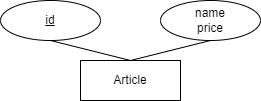
\includegraphics[scale=0.5]{figures/DatabaseER/ArticleServiceTables.png}
	\caption{ER-Diagramm ArticleService}
\end{figure}
\FloatBarrier

\paragraph*{Schnittstellen} \mbox{}\\
% TODO RESTful, Ressource
Die Produktdaten sollen von dem Frontend abgefragt und dargestellt werden. Dabei werden alle vorhandenen Produktdaten selektiert und zurückgegeben. 

Zusätzlich soll der Koordinator eine gezielte Abfrage durchführen können, welche den Preis eines Artikels für eine gegebene ProduktId liefert. Beide Schnittstellen sind RESTful, da jeder Artikel als Ressource angesehen wird. 

Da eine Bestellung mehrere unterschiedliche Artikel enthalten darf, wird zusätzlich eine Schnittstelle angeboten, die dem Aufrufer ermöglicht, mehrere Artikel per Id aufzulösen. Die angefragten ArtikelIds werden als Queryparameter übergeben.

\begin{center}
	\begin{tabular}[h]{|p{3.5cm}|p{3cm}|p{6cm}|}
		\hline
		Endpunkt & Http-Methode & Argumente \\ \hline
		/api/articles & GET & optionale Einschränkung der Ids per Queryparameter \\ \hline
		/api/articles/\{id\} & GET & ArticleId \\ \hline
	\end{tabular}
\end{center}
\FloatBarrier

\subsection{StockService}
\paragraph*{Datenbankschicht} \mbox{}\\

Der StockService verwaltet vier Tabellen. Die zentrale Tabelle ist \textit{articlestock} und stellt für jeden bekannten Artikel den auf Lager befindlichen Vorrat dar. Eine Reservierung für eine gegebene Vorgangsnummer wird in der Tabelle \textit{blockedarticles} durch alle Tupel, bei denen diese Nummer auftritt. Die Lieferungen werden in der Tabelle \textit{shipments} dargestellt. Auch hier gehört eine Vorgangsnummer zu den Spalten. Zusätzlich gibt es das Attribut \textit{hasarrived}, was Auskunft über den Status der Lieferung gibt. Die zu einer Lieferung gehörenden Artikel und deren Menge sind in der Tabelle \textit{shippedarticles} enthalten.

\begin{figure}[h!]
	\centering
	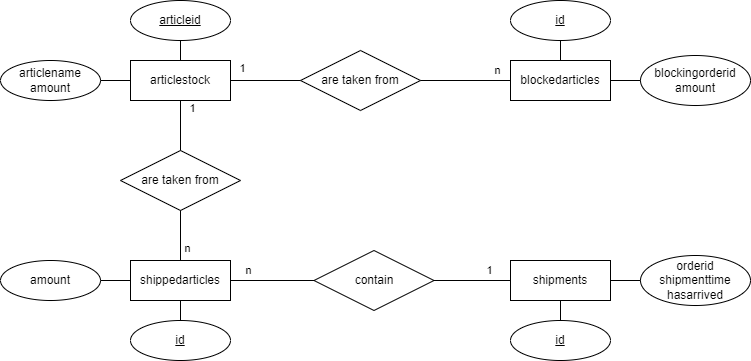
\includegraphics[scale=0.5]{figures/DatabaseER/StockServiceTables.png}
	\caption{ER-Diagramm StockService}
\end{figure}
\FloatBarrier

\paragraph*{Schnittstellen} \mbox{}\\

Der Endpunkt \textit{/api/blocked-articles} überträgt frei verfügbare Artikel aus der Tabelle \textit{articlestock} in die Tabelle \textit{blockedarticles}. Als Argumente werden die zu blockierenden Artikel-Ids und Artikel-Mengen sowie die Vorgangsnummer benötigt. Teil der lokalen Transaktion sind folgende Schritte:
\begin{enumerate}
	\item Reduzieren jedes Artikelvorrats in der Tabelle \textit{articlestock}
	\item Einfügen eines Elements in der Tabelle \textit{blockedarticles} für jede zu blockierende Artikel-Id
\end{enumerate}

Der Endpunkt \textit{/api/blocked-articles-compensation} stellt die Kompensierung für die Schnittstelle \textit{/api/blocked-articles} dar. Als Argument wird hier lediglich die Vorgangsnummer benötigt. Notwendige Schritte der auszuführenden lokalen Transaktion sind:
\begin{enumerate}
	\item Selektieren aller Elemente aus \textit{blocked-articles} mit der angefragten Vorgangsnummer
	\item Löschen dieser Elemente
	\item Erhöhen der Vorratsmengen in \textit{articlestock} für jede Artikelblockierung
\end{enumerate}

Der Endpunkt \textit{/api/start-shipment} erwartet die Vorgangsnummer als Argument. Die reservierten Artikel werden in eine Lieferung umgewandelt und versendet. Die Schritte der ablaufenden lokalen Transaktion sind:
\begin{enumerate}
	\item Initialisieren eines Elements in \textit{shipments} mit dem Status \textit{hasarrived=0}
	\item Selektieren und Löschen aller Elemente in \textit{blockedarticles}, die die OrderId enthalten
	\item Einfügen der Selektierungen in der Tabelle \textit{shippedarticles}
\end{enumerate}

Der Endpunkt \textit{/api/finish-shipment} wird ausschließlich vom Lieferanten verwendet und dient zur Bestätigung der Lieferung. Es wird der Status der entsprechenden ShipmentId in der Tabelle \textit{shipments} auf 1 gesetzt.

Der Endpunkt \textit{/api/shipments} liefert den Status der angeforderten ShipmentId. Der Koordinator hat mit dem Aufruf von \textit{/api/start-shipments} die Lieferung ausgelöst. Der Koordinator hat mit der Schnittstelle \textit{/api/shipments} die Möglichkeit, den Status der Lieferung solange abzufragen, bis der Lieferant per Aufruf von \textit{/api/finish-shipment} den Lieferabschluss bestätigt. Die Kombination von \textit{/api/start-shipment}, \textit{/api/finish-shipment} und \textit{/api/shipments} können als Polling-Implementierung eines asynchronen Request-Response Musters aufgefasst werden. 

Der letzte Endpunkt des StockServices ist \textit{/api/cancel-shipment} und bietet dem Koordinator die Möglichkeit, auf eine Stornierung zu reagieren. Bis die Lieferung abgegeben und bestätigt wurde, kann diese Schnittstelle verwendet werden, um die Lieferung abzubrechen. Als Argument wird die ShipmentId benötigt.

\begin{center}
	\begin{tabular}[h]{|p{6.5cm}|p{3cm}|p{5.1cm}|}
		\hline
		Endpunkt & Http-Methode & Argumente \\ \hline
		/api/blocked-articles & POST & ArticleId, Amount, OrderId\\ \hline
		/api/blocked-articles-compensation & POST & OrderId \\ \hline
		/api/start-shipment & POST & OrderId \\ \hline
		/api/finish-shipment & POST & ShipmentId \\ \hline
		/api/shipments & GET & ShipmentId \\ \hline
		/api/cancel-shipment & POST & ShipmentId \\ \hline
	\end{tabular}
\end{center}
\FloatBarrier

\subsection{BankingService}
\paragraph*{Datenbankschicht} \mbox{}\\
% TODO Tabellenbezeichnungen anpassen
Zur Verwaltung des BankingServices gehören drei Tabellen. Die Tabelle \textit{bankuser} enthält alle Nutzer, die Tabelle \textit{bankusercredit} ordnet jedem Nutzer einen Kontostand zu und die Tabelle \textit{bankusertransaction} stellt Veränderung des Kontostands der Tabelle \textit{bankcredit} in der Tabelle \textit{bankusertransaction} als Historie dar.

\begin{figure}[h!]
	\centering
	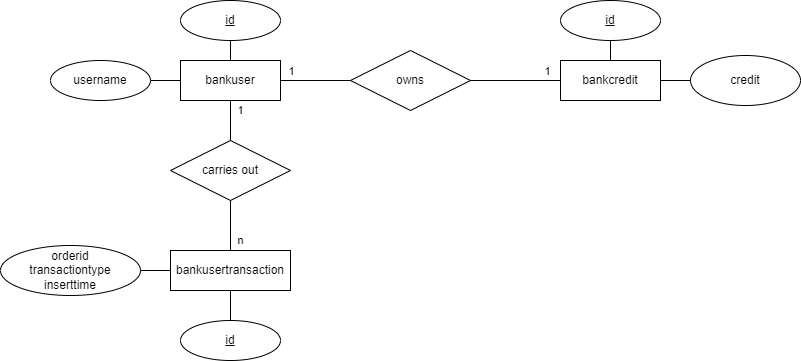
\includegraphics[scale=0.5]{figures/DatabaseER/BankingServiceTables.png}
	\caption{ER-Diagramm BankingService}
\end{figure}
\FloatBarrier

\paragraph*{Schnittstellen} \mbox{}\\
Der BankingService bietet jeweils eine Schnittstelle zum Erhöhen und zum Verringern des Kontostandes an. Dabei wird lediglich in der Tabelle \textit{bankcredit} das Credit-Attribut erhöht oder verringert. Die Spalte ist im Datenbankmanagementsystem mit einer Einschränkung versehen, die verhindert, dass der Wert der Spalte unter 0 fällt. 

Die Veränderung des Kontostandes ist der erste Schritt der lokalen Transaktion. Der zweite Schritt ist das Einfügen eines neuen Elementes in der Tabelle \textit{bankusertransaction}. In dieser Tabelle wird der Transaktionstyp festgehalten. 

\begin{center}
	\begin{tabular}[h]{|l|l|l|}
		\hline
		Endpunkt & Http-Methode & Argumente \\ \hline
		/api/add-money & POST & UserId, Amount, OrderId \\ \hline
		/api/add-money-compensation & POST & UserId, Amount, OrderId \\ \hline
		/api/remove-money & POST & UserId, Amount, OrderId \\ \hline
		/api/remove-money-compensation & POST & UserId, Amount, OrderId \\ \hline 
	\end{tabular}
\end{center}
\FloatBarrier

\section{Ergebnisse}
Der entworfene Prozess soll nun als DEA dargestellt werden. Dafür sind alle möglichen Ergebnisse zu erfassen, die jede lokale Transaktion aus Sicht des Koordinators liefern kann. 

\subsection{Ergebnisse aller Transaktionen}
\begin{center}
	\begin{longtable}[h]{|p{3cm}|p{1.5cm}|p{11cm}|}
		\hline
		Transaktion	& Ergebnis & Bedeutung \\ \hline
		Initialize Saga 	& Success 	& Bestellung ist initialisiert \\ \hline
		Get Article Data	& 200 		& Artikeldaten wurden vom ArticleService empfangen \\
		& 404 		& Artikel wurde nicht gefunden \\ \hline
		Validate Price 		& Success 	& Preis aus Bestellung und aus dem System stimmen überein \\
		& Failure 	& Preise aus Bestellung und aus dem System stimmen nicht überein \\ \hline
		Block Articles		& 200		& Produkte wurden reserviert \\
%		& 208		& Artikel wurden bereits blockiert \\
		& 409 		& Conflict (Lagervorrat ist erschöpft) \\
		& 429 		& Mehrere Transaktionen behindern sich und lokale Transaktion schlägt fehl \\ \hline
		Remove Money 		& 200		& Geldbetrag auf dem Konto wurde verringert \\
%		& 208		& Geldbetrag wurde auf vorherige Anfrage bereits verringert \\
		& 409		& Lokale Transaktion ist fehlgeschlagen (Konto ist nicht gedeckt) \\
		& 429		& Mehrere Transaktionen behindern sich und lokale Transaktion schlägt fehl \\ \hline
		Add Money 			& 200		& Geldbetrag auf dem Konto wurde erhöht \\
%		& 208		& Geldbetrag wurde auf vorherige Anfrage bereits erhöht \\
		& 409		& Lokale Transaktion ist fehlgeschlagen \\
		& 429		& Mehrere Transaktionen behindern sich und lokale Transaktion schlägt fehl \\ \hline
		Start Shipment 		& 200		& Lieferung wurde ausgelöst \\
%		& 208		& Lieferung wurde auf vorherige Anfrage bereits gestartet \\
		& 409		& Lokale Transaktion ist fehlgeschlagen \\
		& 429 		& Mehrere Transaktionen behindern sich und lokale Transaktion schlägt fehl \\ \hline
		Check No Cancellation 	& Success	& Es wurde keine Stornierung festgestellt \\
		& Failure	& Es wurde eine Stornierung festgestellt \\ \hline
		Get Shipment Status	& 200 		& Status wurde vom StockService empfangen \\
		& 404		& Lieferung existiert nicht \\ \hline
		Check Shipment Status & Success	& Lieferstatus signalisiert abgeschlossene Lieferung \\
		& Failure 	& Lieferstatus signalisiert noch nicht abgeschlossene Lieferung \\ \hline
	\end{longtable}
\end{center}
\FloatBarrier

\subsection{Ergebnisse aller Kompensierungen}
\begin{center}
	\begin{longtable}[h]{|p{5.5cm}|p{1.5cm}|p{8.5cm}|}
		\hline
		Transaktion 						& Ergebnis 	& Bedeutung \\ \hline
		Initialize Saga Compensation	 	& Success 	& \\ \hline
		Get Article Data Compensation	 	& Success 	& \\ \hline	
		Validate Price Compensation	 		& Success 	& \\ \hline
		Block Articles Compensation	 		& 200	 	& Reservierung wurde aufgehoben \\
		& 404		& Reservierung wurde nicht gefunden \\
		& 409		& Lokale Transaktion ist fehlgeschlagen \\
		& 429 		& Mehrere Transaktionen behindern sich und lokale Transaktion schlägt fehl \\ \hline
		Remove Money Compensation		 	& 200		& Geldbetrag auf dem Konto wurde erhöht \\
%		& 208		& Transaktion wurde auf vorherige Anfrage bereits kompensiert \\
%		& 404 		& keine zugehörige kompensierbare Transaktion gefunden \\
		& 409		& Lokale Transaktion ist fehlgeschlagen \\
		& 429		& Mehrere Transaktionen behindern sich und lokale Transaktion schlägt fehl \\ \hline
		Add Money Compensation		 		& 200		& Geldbetrag auf dem Konto wurde erhöht \\
		& 208		& Transaktion wurde auf vorherige Anfrage bereits kompensiert \\
		& 404		& keine zugehörige kompensierbare Transaktion gefunden \\
		& 409		& Lokale Transaktion ist fehlgeschlagen \\
		& 429		& Mehrere Transaktionen behindern sich und lokale Transaktion schlägt fehl \\ \hline
		Start Shipment Compensation	 		& 200	 	& Lieferung wurde abgebrochen \\
		& 404		& Lieferung existiert nicht \\
		& 409		& Lokale Transaktion ist fehlgeschlagen \\
		& 410		& Lieferung wurde nicht abgebrochen, da sie bereits abgeschlossen ist \\
		& 429		& Mehrere Transaktionen behindern sich und lokale Transaktion schlägt fehl \\ \hline
	\end{longtable}
\end{center}
\FloatBarrier



\section{Saga Execution Component}

In \ref{sec_Services} wurde festgelegt, dass der OrderService die Rolle des Koordinators übernimmt. Das bedeutet, dass der OrderService die Saga Execution Component enthält. Als solche hat der OrderService die Verantwortung, die an der LLT teilhabenden Services aufzurufen und auf die Ergebnisse zu reagieren. In diesem Abschnitt werden die dafür notwendigen Implementierungsdetails dargestellt.

\subsection{Rahmenbedingung für die Versuchsdurchführung}
Die SEC übernimmt die Aufgabe, einen DEA auszuführen. Im Rahmen des Versuchs sollen mehrere DEAs konstruiert und durch die selbe SEC ausgeführt werden. Die SEC muss also flexibel genug implementiert werden, damit eine Parametrisierung der Ausführung mit einem DEA als Argument möglich ist. 

\subsection{Ausführung eines DEAs}
Zunächste soll der Ablauf eines Durchlaufs eines DEAs innerhalb der SEC dargestellt werden. Es soll nun davon ausgegangen werden, dass ein DEA definiert wurde. 

\begin{enumerate}
	\item Nach Eingang einer Bestellung wird der Initialzustand gewählt, um die Ausführung des DEAs zu starten.
	\item Jeder Zustand korrespondiert mit einer auszuführenden Aktion. Diese Aktion wird ausgeführt. 
	\item Eine Aktion resultiert in einem Ergebnis. Dieses Ergebnis stellt ein Element aus der Menge des Eingabealphabets dar. Dieses Element wird zusammen mit dem Zustand in der Datenbank gespeichert. 
	\item Die Ausführung des Zustands wird beendet.
	\item Die SEC bestimmt den nächsten Zustand. Und führt die korrespondierende Aktion aus.
	\item Die Aktion resultiert in einem Ergebnis. Das Ergebnis wird in der Datenbank gespeichert. 
	\item Die Ausführung des Zustands wird beendet. 
	\item Die SEC wiederholt diesen Prozess solange bis ein Endzustand erreicht wird. 
\end{enumerate}

\subsection{Modellierung eines DEAs}
Die Modellierung eines DEAs ist in \cref{lst:dea-model-csharp} abgebildet. 

\begin{lstlisting}[breaklines=true, tabsize=2, showstringspaces=false, frame=single, numbers=left, basicstyle=\small, label = {lst:dea-model-csharp}, caption={Modellierung eines DEA in C\#}, captionpos=b] 
public class SimpleStateMachine
{
	public List<string> States;
	public string InitialState;
	public List<string> EndStates;
	public List<string> Sigma;
	public List<Tuple<Tuple<string, string>, string>> Relations;
	
	
	public SimpleStateMachine(List<string> states,
		string initialState,
		List<string> endStates,
		List<string> sigma,
		List<Tuple<Tuple<string, string>, string>> relations)
	{
		States = states;
		InitialState = initialState;
		EndStates = endStates;
		Sigma = sigma;
		Relations = relations;
	}
}
\end{lstlisting}

\paragraph*{Relations} \mbox{}\\
Das Feld \textit{Relations} stellt Liste von möglichen Zustandsübergängen dar. Die SEC kann aus einem Zustand und einem Element aus Sigma den entsprechenden Zustandsübergang berechnen. Damit diese Berechnung deterministisch ist, darf für einen gegebenen Zustand und einen gegebenes Element aus Sigma nur ein Element existieren. 

\subsection{Konstruktion eines DEAs}
Nun soll ein solcher DEA initialisiert werden. Dazu wird der Konstruktor dieser Klasse aufgerufen. Es soll folgender Automat konstruiert werden:

\begin{figure}[ht!]
	\centering
	\begin{tikzpicture}[->,>=stealth',shorten >=1pt,auto,node distance=2.5cm, semithick]
		\node [state, initial] 		(qt1) 					{$q_{t1}$};
		\node [state] 				(qt2) [right of=qt1] 	{$q_{t2}$};
		\node [state] 				(qt3) [right of=qt2] 	{$q_{t3}$};
		
		\node [state] 				(qc1) [below of=qt2] 	{$q_{c1}$};
		\node [state] 				(qc2) [right of=qc1] 	{$q_{c2}$};
		
		\node [state, accepting] 	(qf1) [right of=qt3] 	{$q_{f1}$};
		\node [state, accepting] 	(qf2) [left of=qc1] 	{$q_{f2}$};
		\node [state, accepting] 	(qf3) [below of=qc2] 	{$q_{f3}$};
		
		\path (qt1) 	edge					node 		{$t1_{200}$}		(qt2)
						edge					node		{$t1_{400}$}		(qf2)
		(qt2)			edge					node		{$t2_{Success}$}	(qt3)
						edge					node		{$t2_{Failure}$}	(qc1)
		(qt3)			edge					node		{$t3_{200}$}		(qf1)
						edge					node		{$t3_{400}$}		(qc2)
		(qc1)			edge					node		{$c1_{200}$}		(qf2)
						edge	[bend right]	node		{$c1_{400}$}		(qf3)
		(qc2)			edge					node		{$c2_{Success}$}	(qc1)
						edge					node		{$c2_{Failure}$}	(qf3);
	\end{tikzpicture}
	\caption{Zu konstruierender DEA}
\end{figure}
\FloatBarrier

Die Initialisierung ist in \cref{lst:dea-model-example-csharp} abgebildet:

\begin{lstlisting}[language={[Sharp]C}, breaklines=true, tabsize=2, showstringspaces=false, frame=single, numbers=left, basicstyle=\small,label = {lst:dea-model-example-csharp}, caption={Modellierung eines Beispiel DEA in C\#}, captionpos=b] 
public class ExampleDea
{
 	// representation of states
	public static string Q_T1 = "qt1";
	public static string Q_T2 = "qt2";
	public static string Q_T3 = "qt3";
	public static string Q_C1 = "qc1";
	public static string Q_C2 = "qc2";
	public static string Q_F1 = "qf1";
	public static string Q_F2 = "qf2";
	public static string Q_F3 = "qf3";
	
	// representation of sigma
	public static string T1_200 = "t1_200";
	public static string T1_400 = "t1_400";
	public static string T2_Success = "t2_Success";
	public static string T2_Failure = "t2_Failure";
	public static string T3_200 = "t3_200";
	public static string T3_400 = "t3_400";
	public static string C1_200 = "c1_200";
	public static string C1_400 = "c1_400";
	public static string C2_200 = "c2_200";
	public static string C2_400 = "c2_400";
	
	public SimpleStateMachine ConstructExampleDea()
	{
		var states = new List<string>
		{
			Q_T1, Q_T2, Q_T3, Q_C1, Q_C2, Q_F1, Q_F2, Q_F3,
		};
		
		var initialState = qt1;
		
		var sigmaElements = new List<string>
		{
			T1_200, T1_400,
			T2_Success, T2_Failure,
			T3_200, T3_400,
			C1_200, C1_400,
			C2_200, C2_400
		};
		
		var endStates = new List<string>
		{
			Q_F1, Q_F2, Q_F3
		};
		
		var relations = new List<
			Tuple<Tuple<string, string>, string>>
		{
			BuildRelation(Q_T1, T1_200, Q_T2),
			BuildRelation(Q_T1, T1_400, Q_F2),
			BuildRelation(Q_T2, T2_Success, Q_T3),
			BuildRelation(Q_T2, T2_Failure, Q_C1),
			BuildRelation(Q_T3, T3_200, Q_F1),
			BuildRelation(Q_T3, T3_400, Q_C2),
			BuildRelation(Q_C1, C1_200, Q_F2),
			BuildRelation(Q_C1, C1_400, Q_F3),
			BuildRelation(Q_C2, C2_200, Q_C1),
			BuildRelation(Q_C2, C2_400, Q_F3)
		};
		
		return new SimpleStateMachine(states, initialState, sigmaElements, endStates, relations); 
	}
	
	private Tuple<Tuple<string, string>, string> BuildRelation(
		string inputState, 
		string inputSigmaElement, 
		string newState)
	{
		return new Tuple<Tuple<string, string>, string>(
			new Tuple<string, string>(inputState, inputSigmaElement), 
		newState);
	}
}
\end{lstlisting}

\paragraph*{Verwaltung der DEAs} \mbox{}\\
Nach Vorbild des Beispiels in \cref{lst:dea-model-example-csharp} werden alle ausführbaren DEAs definiert. Diese Initialisierung geschieht innerhalb der in \cref{lst:statemachinemapper-csharp} definierten Klasse. 

\begin{lstlisting}[language={[Sharp]C}, breaklines=true, tabsize=2, showstringspaces=false, frame=single, numbers=left, basicstyle=\small,label = {lst:statemachinemapper-csharp}, caption={Modellierung eines StateMachineMappers in C\#}, captionpos=b] 
public interface IStateMachineMapper 
{
	StateMachine MapToStateMachine(int smValue);
}

public class StateMachineMapper : IStateMachineMapper
{
	private readonly StateMachine Sm1;
	private readonly StateMachine Sm2;
	// more StateMachineDefinitions
	
	public StateMachine MapToStateMachine(int smValue) {
		switch (smValue) 
		{
			case 1:
				return Sm1;
			case 2: 
				return Sm2;
			// ...
		}
		
        throw new UnknownStateMachineException($"Unknown StateMachine for value [{smValue}].");
	}
	
}
\end{lstlisting}

Per Dependency Injection kann die SEC diese Klasse verwenden. Per Strategie-Pattern wird in einer Funktion der gewünschte DEA ermittelt werden.

\paragraph*{Kontrollfluss der SEC} \mbox{}\\
Die SEC verwendet den StateMachineMapper, um den gewünschten DEA auszuführen. Die tatsächliche Ausführung findet in einer separaten Komponente, dem StateMachineExecutor statt. Diese Klasse enthält eine Funktion \textit{ExecuteStateMachine}, die für einen DEA und ein Eingabewort den aktuellen Zustand berechnet. Dazu wird jedes Element des Eingabeworts abgearbeitet. Für jedes Element und den aktuellen Zustand wird in der Funktion \textit{FindRelation} die zugeordnete Relation berechnet. Der in der Relation enthaltene Folgezustand wird gesetzt und das abgearbeitete Element des Eingabeworts wird entfernt. 

Das Ergebnis der Berechnung ist eine Liste von Konfigurationsübergängen. Eine Konfiguration wird durch die in \cref{lst:statemachineconfiguration-csharp} dargestellten Klasse modelliert.

\begin{lstlisting}[language={[Sharp]C}, breaklines=true, tabsize=2, showstringspaces=false, frame=single, numbers=left, basicstyle=\small,label = {lst:statemachineconfiguration-csharp}, caption={Modellierung einer StateMachineConfiguration in C\#}, captionpos=b] 
public class StateMachineConfiguration
{
	public List<string> Word { get; set; } = new();
	public string State { get; set; } = string.Empty;
	
	// Clone Function
}
\end{lstlisting}

Ein Konfigurationsübergang stellt den Wechsel von einer Konfiguration in eine Folgekonfiguration dar. Dabei wird die Länge des Eingabeworts stets verringert.

\begin{lstlisting}[language={[Sharp]C}, breaklines=true, tabsize=2, showstringspaces=false, frame=single, numbers=left, basicstyle=\small,label = {lst:statemachineconfigurationtransition-csharp}, caption={Modellierung einer StateMachineConfigurationTransition in C\#}, captionpos=b] 
public class StateMachineConfigurationTransition
{
	public StateMachineConfiguration C1 { get; set; }
	public StateMachineConfiguration C2 { get; set; }
	public Tuple<Tuple<string, Status>, string> Relation { get; set; }
	
	public StateMachineConfigurationTransition(
		StateMachineConfiguration c1, 
		StateMachineConfiguration c2, 
		Tuple<Tuple<string, string>, string> relation)
	{
		C1 = c1;
		C2 = c2;
		Relation = relation;
	}
}
\end{lstlisting}

Solange das Eingabewort noch nicht vollständig abgearbeitet wurde, werden Konfigurationsübergänge berechnet. Die resultierende Liste von Konfigurationsübergängen beschreibt eindeutig den gewählten Graphen. 

\begin{lstlisting}[language={[Sharp]C}, breaklines=true, tabsize=2, showstringspaces=false, frame=single, numbers=left, basicstyle=\small,label = {lst:statemachineexecutor-csharp}, caption={Modellierung einer StateMachineExecutors in C\#}, captionpos=b] 
public interface IStateMachineExecutor
{
	List<StateMachineConfigurationTransition> ExecuteStateMachine(StateMachine sm, List<Status> word);
}

public class StateMachineExecutor : IStateMachineExecutor
{
	public List<StateMachineConfigurationTransition> ExecuteStateMachine(StateMachine sm, List<string> word)
	{
		List<StateMachineConfigurationTransition> result = new();
		
		StateMachineConfiguration current = new StateMachineConfiguration
		{
			Word = word,
			State = sm.InitialState
		};
		
		while (current.Word.Count > 0)
		{
			StateMachineConfiguration c1 = StateMachineConfiguration.Clone(current);
			
			var relation = FindRelation(sm.Relations, current);
			
			string nextState = relation.Item2;
						
			current.State = nextState!;
			current.Word.RemoveAt(0);
			
			StateMachineConfigurationTransition transition = new()
			{
				C1 = c1,
				C2 = new StateMachineConfiguration
				{
					State = nextState,
					Word = current.Word
				},
				Relation = relation
			};
			
			result.Add(transition);
		}
		
		return result;
	}
	
	private Tuple<Tuple<string, string>, string> FindRelation(
		List<Tuple<Tuple<string, string>, string>> relations, 	
		StateMachineConfiguration currentConfiguration)
	{
		foreach (var relation in relations)
		{
			var relStartState = relation.Item1.Item1;
			var relWord = relation.Item1.Item2;
			
			if (currentConfiguration.State.Equals(relStartState) && 
				currentConfiguration.Word.First() == relWord)
			{
				return relation;
			}
		}
		
		throw new NoRelationException($"No Relation found for State = [{currentConfiguration.State}] and Element = [{currentConfiguration.Word.First()}]");
	}
}
\end{lstlisting}

Das Ergebnis der Berechnung ist die Liste von Konfigurationsübergängen. Der letzte Konfigurationsübergang enthält den Zielzustand, der noch auszuführen ist. Über den ActionExecutor wird die mit diesem Zustand korrespondierende Aktion ausgeführt. Die Kommunikation der von der SEC verwendeten Klassen ist in \cref{fig:sequence_diagramm_sec_control_flow} abgebildet. 

Die Funktion \textit{GetTransactionsForOrderSaga} greift auf die Datenbanktabelle \textit{ordersagatransactions} zu und liefert das Transaktionslog. Das Transaktionslog wird lediglich von den mit einem Zustand korrespondierenden Aktionen ergänzt. Die SEC selbst greift nur lesend auf dieses Log zu.

\begin{figure}[H]
	\centering
	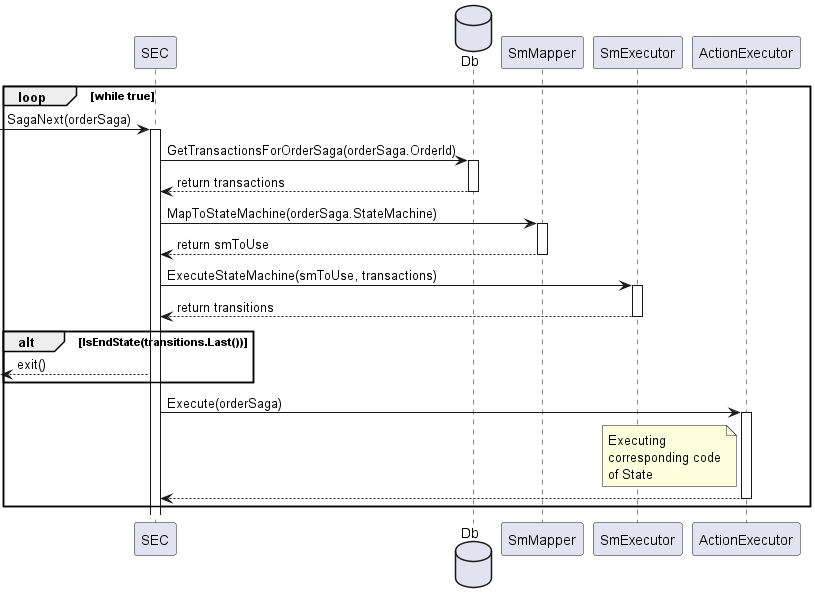
\includegraphics[width=\linewidth]{figures/ChapterVersuchsdurchführung/sec_execution_flow.png}
	\caption{Kontrollfluss der SEC}
	\label{fig:sequence_diagramm_sec_control_flow}
\end{figure}
\FloatBarrier


\section{Planung der Datenerfassung}
Auf Grundlage des nun bekannten Systems sollen die Testfälle und Testszenarien definiert werden.

\subsection{Testszenarien}
Ein Testszenario soll das Verhalten des Netztwerks beschreiben. Ziel der in diesem Kapitel stattfindenden Untersuchung ist eine robuste Saga-Implementierung, die in allen möglichen Testszenarien ein konsistentes Verhalten des Systems gewährleistet. 

\subsection{Fehlerquellen}
Zuerst ist zu identifizieren, an welchen Stellen eine Kommunikation in einem verteilten System mittels Request-Response-Muster fehlschlagen kann. Im folgenden Beispiel wird dies anhand einer simplen Kommunikation illustriert, die aus einem Request und einer Response besteht. Es wird davon ausgegangen, dass die Verarbeitung des Requests zu einer Änderung des Systemzustands des Empfängers führt. 

\paragraph*{Szenario 1}
Im ersten Szenario entstehen keine Netzwerkfehler. Dieses Szenario ist der Ausgangspunkt. Die Korrektheit der Saga in diesem Fall ist eine Voraussetzung für die Formulierung und Analyse in folgenden Szenarien. 

\begin{figure}[H]
	\centering
	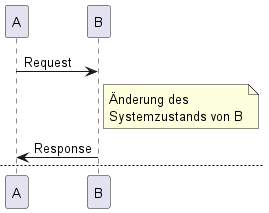
\includegraphics[width=.4\linewidth]{figures/ChapterVersuchsvorbereitung/TestSzenarien-0.png}
	\label{fig:Testszenario1}
	\caption{Szenario 1}
\end{figure}
\FloatBarrier

\paragraph*{Szenario 2}
Es können Netzwerkfehler auftreten, die verhindern, dass der Request den Empfänger erreicht. Dabei findet keine Verarbeitung der Nachricht im Empfängerservice statt. Es findet weder eine Veränderung des Systemzustands des Empfängers noch eine Versendung einer Response statt.

\begin{figure}[H]
	\centering
	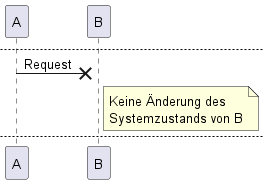
\includegraphics[width=.4\linewidth]{figures/ChapterVersuchsvorbereitung/TestSzenarien-1.png}
	\label{fig:Testszenario2}
	\caption{Szenario 2}
\end{figure}
\FloatBarrier

Im Rahmen dieses Versuchs wird das Auftreten solcher Fehler in Testszenario 2 simuliert. 

\paragraph*{Szenario 3}
Findet ein Netzwerkfehler nach der Verarbeitung des Requests im Empfängerservice statt, erreicht die Response den Sender nicht. Die abgeschlossene Verarbeitung des Requests hat zu einer Veränderung des Systemzustands im Empfängerservice geführt. Dies führt dazu, dass der Sender keine Kenntnis über den Erfolg oder Misserfolg des ursprünglichen Requests hat.

\begin{figure}[H]
	\centering
	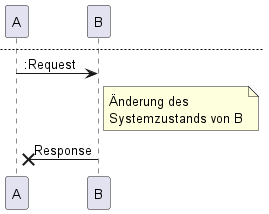
\includegraphics[width=.4\linewidth]{figures/ChapterVersuchsvorbereitung/TestSzenarien-2.png}
	\label{fig:Testszenario3}
	\caption{Szenario 3}
\end{figure}
\FloatBarrier

Im Rahmen dieses Versuchs wird das Auftreten solcher Fehler in Testszenario 3 simuliert. Zusätzlich treten in Testszenario 3 die Netzwerkfehler des Testszenario 2 auf. 

Das Testszenario 3 simuliert somit ein Netzwerkverhalten, welches verschiedene Arten von Netzwerkfehlern abdeckt. Wenn eine LLT unter den im Testszenario 3 geschaffenen Bedingungen Konsistenz gewährt, kann die These angenommen werden.

% TODO

\subsection{Simulation der Testfälle}
Die zu simulierenden Testfälle werden durch einen separaten Service durchgeführt, die TestApi. Die Schnittstellen, die direkt mit der Durchführung der LLT interagieren sind:

\begin{center}
	\begin{longtable}[h]{|p{2.3cm}|p{4.9cm}|p{3.2cm}|p{3.4cm}|}
		\hline
		Service & Schnittstelle & Beschreibung & Akteur \\ \hline
		OrderService & \textit{POST /api/orders} & Platzieren einer Bestellung & Frontend (Kunde) \\ \hline
		StockService & \textit{POST /api/finish-shipment} & Lieferbestätigung & Lieferant \\ \hline
		OrderService & \textit{POST /api/cancel-order} & Stornierung & Frontend (Kunde) \\ \hline
	\end{longtable}
\end{center}
\FloatBarrier

\paragraph*{FinishOrders}
Der erste Testfall simuliert eine erfolgreiche Verarbeitung des Bestell- und Lieferprozesses. Die TestApi generiert Bestellungen und ruft den entsprechenden Endpunkt zum Platzieren im OrderService auf. Für jede der Bestellungen wird in der TestApi gewartet, bis die Lieferung ausgelöst wurde. Dann wird die Lieferbestätigung simuliert, indem der entsprechende Endpunkt im StockService aufgerufen wird. 

Der Koordinator erhält die Möglichkeit, den erfolgreichen Endzustand zu erreichen. Dies ist der erwartete Endzustand. Dieser Testfall wird als \textit{FinishOrders} bezeichnet. 

\paragraph*{CancelOrders}
Der zweite Testfall simuliert eine Stornierung der Bestellung. Die TestApi generiert Bestellungen und platziert diese. Nachdem die Lieferung ausgelöst wurde, platziert die TestApi die Stornierung. 

Der Koordinator erkennt die Stornierung und hat die Verantwortung, die Lieferung zu stoppen und im Anschluss alle lokalen Transaktionen zu kompensieren. In diesem Testfall werden alle Kompensierungen aufgerufen. Dieser Testfall wird mit \textit{CancelOrders} bezeichnet. 

Der erwartete Endzustand dieser Bestellung ist \textit{FailedWithCompensation}.
\subsection{Datengenerierung}
Um den Ablauf der Services zu simulieren, müssen Daten in jedem Teilsystem generiert werden. Dabei wird in dieser Versuchsdurchführung zwischen zwei Arten der Datengenerierung unterschieden: statische und dynamische Datengenerierung.

\paragraph*{Statisch generierte Daten}
Zu den statisch generierten Daten gehören die Daten, die manuell einmalig generiert und anschließend in die Datenbank eingefügt werden.

Im ArticleService werden die Daten der Produkttabelle generiert. Dazu gehören die verschiedenen Produktbezeichnungen und Preise.

In den zwei BankServices werden die Daten der Nutzertabellen generiert. Für jeden BankService werden 100 verschiedene Nutzer erstellt. Initial erhält jeder dieser Nutzer einen ausreichend großen Geldbetrag als Startguthaben. 

\paragraph*{Dynamisch generierte Daten}
Die in der TestApi generierten Bestellungen werden dynamisch erzeugt. Jede Bestellung wählt einen zufälligen BankService-Nutzer und eine Menge von zwischen 1 und 10 verschiedenen Artikeln mit einer zufälligen Menge zwischen 1 und 4.

Eine solche zufällig generierte Bestellung ist in \cref{lst:PlaceOrderJson} abgebildet.


\begin{lstlisting}[breaklines=true, tabsize=2, showstringspaces=false, frame=single, numbers=left, basicstyle=\small, label = {lst:PlaceOrderJson}, caption={Dynamisch generierte Bestellung}, captionpos=b] 
{
	"consument": {
		"userId": "Xena",
		"bankId": "Bank1"
	},
	"requestedArticles": [
	{
		"articleId": 42,
		"articlePrice": 99.0,
		"amount": 2
	},
	{
		"articleId": 16,
		"articlePrice": 49.99,
		"amount": 3
	}
}
\end{lstlisting}

\subsection{Messwerte}
Um die verschiedenen Messungen vergleichen zu können, werden die Messungen eines DEAs in jedem Testfall und in jedem Testszenario durchgeführt. Nach der Messung sollen daraus Aussagen über die Konsistenz und über die Korrektheit der modellierten LLT getroffen werden. Dazu werden folgende Messwerte erhoben:

\paragraph*{StateAnalysisResult}
Dieser Teil des Messergebnisses verwendet die im Koordinator enthaltenen Zustände. Als Scope wird ein konkreter Testfall, ein konkretes Testszenario und ein DEA festgelegt.

\begin{center}
\begin{longtable}[h]{|p{5cm}|p{12cm}|}
	\hline
	Messwert & Beschreibung \\ \hline
	totalCount & Anzahl der Sagas \\ \hline
	successfullCount & Anzahl der Sagas mit Endzustand $q_{Success}$ \\ \hline
	finishedCount & Anzahl der Sagas mit Endzustand $\not = q_{Pending}$ \\ \hline
	pendingCount & Anzahl der Sagas mit Endzustand $q_{Pending}$ \\ \hline
	failedWithCompensation\-Count & Anzahl der Sagas mit Endzustand $q_{failedWithCompensation}$ \\ \hline
	failedWithoutCompensation\-Count & Anzahl der Sagas mit Endzustand $q_{failedWithoutCompensationCount}$ \\ \hline
	hasCorrectEndstateCount & Anzahl der Sagas mit dem erwarteten Endzustand des Testfalls \\ \hline
	containsAllExpectedLogs\-Count & Anzahl der Sagas, deren Transaktionslog alle erwarteten Logs des Testfalls aufweist \\ \hline
	isSuccessfullTestInstance\-Count & Anzahl der Sagas mit dem erwarteten Endzustand und erwarteten Transaktionslogs des Testfalls \\ \hline
\end{longtable}
\end{center}
\FloatBarrier

Für jeden dieser Werte gibt wir einen normalisierter Wert berechnet, der ins Verhältnis zum Messwert \textit{totalCount} gesetzt wird. Da diese Werte ausschließlich aus der Sicht des Koordinators gemessen werden, geben diese Werte lediglich Auskunft über den erreichten Endzustand einer Saga. Eine Saga mit dem Endzustand $q_{Success}$ ist nicht gleichbedeutend mit einer konsistenten LLT. 

\paragraph*{TransactionAnalysisResult}
Um Aussagen über die Konsistenz einer LLT zu treffen, werden die durchgeführten Transaktionen, die im Transaktionslog des Koordinators festgehalten sind, mit den durchgeführten Transaktionen der Teilnehmerservices verglichen. Für jede Saga kann der Unterschied zwischen Transaktionsanzahl aus Koordinatorsicht und aus Teilnehmerservicesicht berechnet werden. Enthält eine Saga mindestens eine Transaktion, bei der dieser Unterschied auftritt, wird sie als inkonsistent bezeichnet. Die Summe der Unterschiede pro Transaktionstyp kann ebenfalls gebildet werden. Es ergibt sich folgende Tabelle:

\begin{center}
	\begin{longtable}[h]{|p{5cm}|p{12cm}|}
		\hline
		Messwert & Beschreibung \\ \hline
		diffRemoveMoney\-Transaction & Summe der Unterschiede über alle Sagas für Transaktionstyp RemoveMoney \\ \hline
		diffAddMoney\-Transaction & Summe der Unterschiede über alle Sagas für Transaktionstyp AddMoney \\ \hline
		diffRemoveMoney\-CompensationTransaction &  Summe der Unterschiede über alle Sagas für Transaktionstyp RemoveMoneyCompensation \\ \hline
		diffAddMoney\-CompensationTransaction &  Summe der Unterschiede über alle Sagas für Transaktionstyp AddMoneyCompensation \\ \hline
		diffBlockArticles\-Transaction &  Summe der Unterschiede über alle Sagas für Transaktionstyp BlockArticles \\ \hline
		diffStartShipment\-Transaction &  Summe der Unterschiede über alle Sagas für Transaktionstyp StartShipment \\ \hline
		diffBlockArticles\-CompensationTransaction &  Summe der Unterschiede über alle Sagas für Transaktionstyp BlockArticlesCompensation\\ \hline
		diffStartShipment\-CompensationTransaction &  Summe der Unterschiede über alle Sagas für Transaktionstyp StartShipmentCompensation\\ \hline
		consistentSagas & Anzahl der konsistenten Sagas \\ \hline	
	\end{longtable}
\end{center}
\FloatBarrier

\paragraph*{ExecutionTimeAnalysisResult}
Schlussendlich wird ein weiteres Messergebnis definiert. Dieses Ergebnis dient dazu, die verschiedenen DEAs hinsichtlich ihrer Laufzeit zu untersuchen. Dabei wird die Differenz der ersten und letzten Transaktion im Log des Koordinators gebildet. 

\begin{center}
	\begin{longtable}[h]{|p{5cm}|p{12cm}|}
		\hline
		Messwert & Beschreibung \\ \hline
		minRuntime & minimale Laufzeit aller Sagas [s]\\ \hline
		maxRuntime & maximale Laufzeit aller Sagas [s]\\ \hline
		avgRuntime & durchschnittliche Laufzeit aller Sagas [s]\\ \hline
		medianRuntime & 50\% Quantil der Laufzeit aller Sagas [s]\\ \hline
		upperQuartileRuntime & 75\% Quantil aller Sagas [s]\\ \hline
		lowerQuartileRuntime & 25\% Quantil aller Sagas [s]\\ \hline
\end{longtable}
\end{center}
\FloatBarrier

Die Analyse der Laufzeiten trägt keine Bedeutung für Aussagen bezüglich der Konsistenz oder Korrektheit einer LLT. Ein wesentliches Werkzeug für die Definition der verschiedenen DEAs sind Retries. Die ExecutionTimeAnalysisResults geben Auskunft, inwiefern die Laufzeit einer Saga beeinflusst wird.

\section{Implementierung des SmBasic}

Der DEA der ersten Implementierung wird im Folgenden als SmBasic bezeichnet. Dieser DEA soll das grundlegende Prinzip des Saga-Patterns unter Verwendung der Backward-Recovery implementieren. Jeglicher Fehler führt dazu, dass die SEC eine Kompensierung der Saga verfolgt.

\subsection{Strategie für die Konstruierung des DEAs SmBasic}

Alle Erfolge eines Ts führen zum folgenden T. Alle anderen Ergebnisse führen für Ts zu einem Zustandswechsel zu dem nächstkleineren C. Erfolgreiche Cs führen zum nächstkleinerem C. Alle anderen Ergebnisse führen für Cs zu einem Zustandswechsel in den Zustand \textit{FailedWithCompensation}. Das letzte T führt bei Erfolg zu einem Übergang in den Zustand \textit{Done}. Ebenso führt $C_1$ bei Erfolg zu einem Übergang in den Zustand \textit{FailedWithCompensation}. 

\begin{center}
	\begin{longtable}[h]{|p{2.6cm}|p{2cm}|p{2.8cm}|p{5cm}|}
		\hline
		Ergebnistyp & Zustand & Ergebnis $e$& Folgezustand \\ \hline
		API-Ergebnis & $T_n$ & $e \in \{Tn_{200}\}$ & $T_{n+1}$ \\ \hline
		API-Ergebnis & $T_n$ & $e \not\in \{Tn_{200}\}$ & $C_{n-1}$ \\ \hline
		IPE & $T_n$ & $e \in \{Tn_{Success}\}$ & $T_{n+1}$\\ \hline
		IPE & $T_n$ & $e \not\in \{Tn_{Success}\}$ & $C_{n-1}$\\ \hline
		API-Ergebnis & $C_n$ & $e \in \{Cn_{200}\}$ & $C_{n-1}$ \\ \hline
		API-Ergebnis & $C_n$ & $e \not\in \{Cn_{200}\}$ & \textit{FailedWithoutCompensation} \\ \hline
		IPE & $C_n$ & $e \in \{Cn_{Success}\}$ & $C_{n-1}$\\ \hline
		IPE & $C_n$ & $e \not\in \{Cn_{Success}\}$ & \textit{FailedWithoutCompensation}\\ \hline
	\end{longtable}
\end{center}
\FloatBarrier

Aus diesem Regelwerk ergibt sich der in \cref{fig:fig_sm_basic} dargestellte DEA. 

\begin{figure}[H]
	\centering
	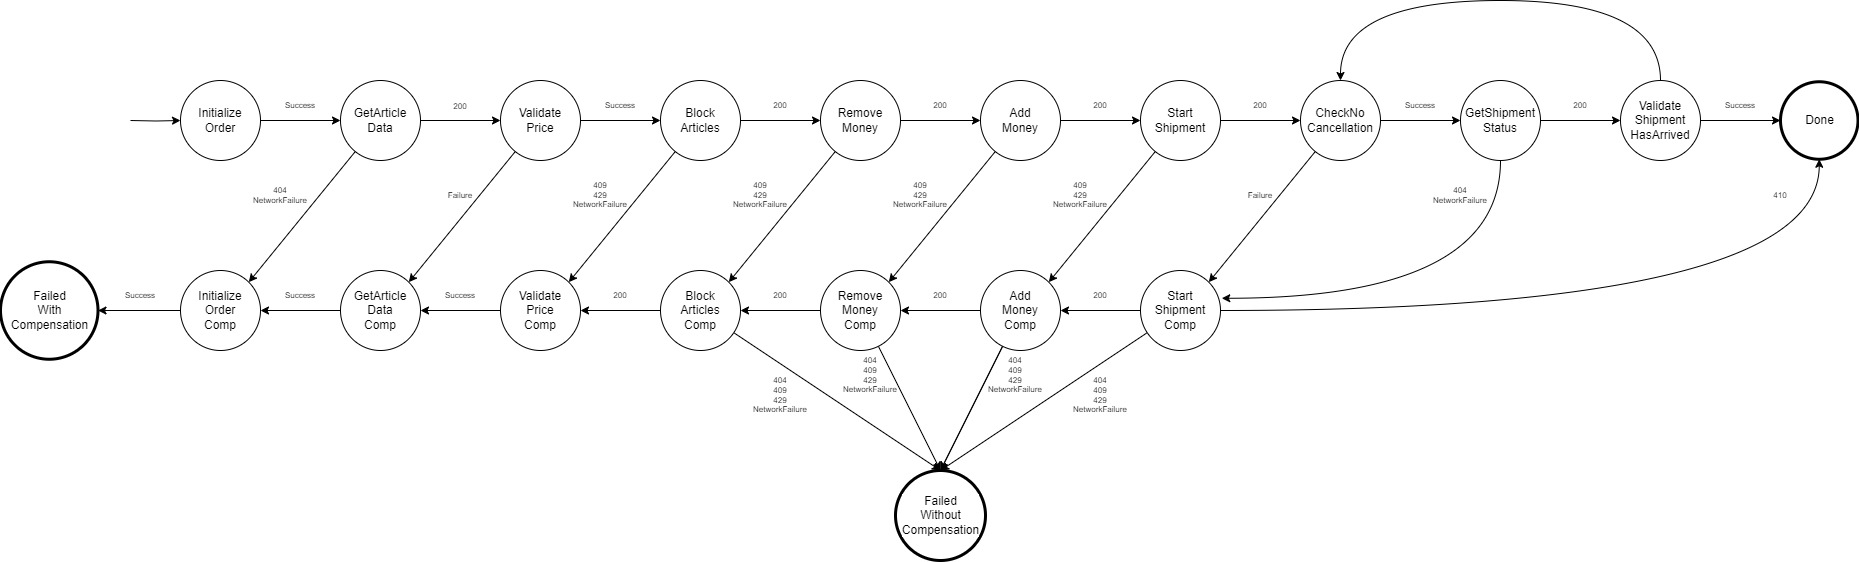
\includegraphics[width=\linewidth]{figures/ChapterVersuchsdurchführung/sm_basic.jpg}
	\caption{DEA für SmBasic}
	\label{fig:fig_sm_basic}
\end{figure}
\FloatBarrier

\subsection{StateAnalysisResult}

\paragraph*{Testfall FinishOrders} \mbox{}\\
Folgende Tabelle bildet das StateAnalysisResult der Messung des SmBasic in Testfall FinishOrders.

\begin{center}
	\fontsize{9}{12}\selectfont
	\begin{longtable}[h]{|p{5cm}|p{1cm}|p{1cm}|p{1cm}|}
		\hline
		Messwert & S1 & S2 & S3 \\ \hline
		\endhead
		%\label{tab:smbasic_stateanalysisresult_finishorders}
		\endfoot
		successfull\-Percentage & 0.80 & 0.42 & 0.19 \\ \hline
		finished\-Percentage & 1.0 & 1.0 & 1.0 \\ \hline
		pending\-Percentage & 0.0 & 0.0 & 0.0 \\ \hline
		failedWithCompensation\-Percentage & 0.20 & 0.53 & 0.72 \\ \hline
		failedWithoutCompensation\-Percentage & 0.0 & 0.06 & 0.10 \\ \hline
		hasCorrectEndstate\-Percentage & 0.80 & 0.42 & 0.19 \\ \hline
		containsAllExpectedLogs\-Percentage & 0.80 & 0.38 & 0.15 \\ \hline
		isSuccessfullTestInstance\-Percentage & 0.80 & 0.38 & 0.15 \\ \hline
	\end{longtable}
\end{center}
\FloatBarrier

Die Messung zeigt, dass bereits in Testszenario 1 nur 80\% der Sagas zum erwarteten Endzustand führen. Der Anteil der Sagas, die den Zustand \textit{Success} erreichen, wird mit jedem Testszenario geringer: 80\% in Testszenario S1, 42\% in S2 und 19\% in S3.

Das ist damit zu begründen, dass jeglicher Fehler in der Ausführung des SmBasic zur Kompensierung führt. Zu den Fehlern, die zur Kompensierung (für Ts) oder zum Zustand \textit{FailedWithoutCompensation} (für Cs) führen, gehören neben den Fehlern, die einen kritischen Konflikt ausdrücken auch vorübergehende Fehler (API-Ergebnisse mit $tn_{429}$) und in S2 und S3 Netzwerkfehler. 

Dies drückt sich außerdem in dem Messwert \textit{failedWithoutCompensation} aus, der ebenfalls in jedem Testszenario größer wird.

In \cref{tab:transaktionslog_ts1_tc1_429} ist das Transaktionslog einer Saga abgebildet, die aufgrund eines vorübergehenden Fehlers abgebrochen wurde. 

\begin{center}
	\fontsize{9}{12}\selectfont
	\begin{longtable}[h]{|p{4.5cm}|p{7cm}|}
		\hline
		Zustand & Ergebnis \\* \hline
		\endhead
		\hline
		\caption{Transaktionslog für Saga im Testfall 1 und Testszenario 1}
		\label{tab:transaktionslog_ts1_tc1_429}
		\endfoot
  		InitializeOrder & InitializeSagaSuccess \\* \hline
		GetArticleData & GetProductData200 \\* \hline
		ValidatePrice & ValidatePriceSuccess \\* \hline
		\rowcolor{Gray}
		BlockArticles & BlockArticles429 \\* \hline
		ValidatePriceCompensation & ValidatePriceCompensationSuccess \\* \hline
		GetArticleDataCompensation & GetProductDataCompensationSuccess \\* \hline
		InitializeOrderCompensation & InitializeSagaCompensationSuccess \\* \hline
	\end{longtable}
\end{center}
\FloatBarrier

\paragraph*{Testfall CancelOrders} \mbox{}\\
In \cref{tab:smbasic_stateanalysisresult_cancelorders} ist das StateAnalysisResult für den Testfall CancelOrders dargestellt. Hier zeigt sich die Berechtigung des Messwertes \textit{isSuccessfullTestInstancePercentage}. Der erwartete Endzustand \textit{FailedWithCompensation} wird in diesem Testfall erwartet und in Testszenario 1 in 95\% aller Sagas erreicht. Der Messwert \textit{containsAllExpectedLogsPercentage} zeigt, dass in Testszenario 1 lediglich 87\% die erwarteten Logs enthalten. Das bedeutet, dass ein Anteil der Sagas mit Endzustand \textit{FailedWithCompensation} aufgrund eines Fehlers zur Kompensierung gewechselt haben und nicht wie erwartet den Zustand \textit{CheckNoCancellation} erreicht haben. Somit stellen diese Sagas keine erfolgreichen Testinstanzen mehr dar.

\begin{center}
	\fontsize{9}{12}\selectfont
	\begin{longtable}[h]{|p{5cm}|p{1cm}|p{1cm}|p{1cm}|}
		\hline
		Messwert & S1 & S2 & S3 \\ \hline
		\endhead
		%\label{tab:smbasic_stateanalysisresult_cancelorders}
		\endfoot
		successfull\-Percentage & 0.0 & 0.0 & 0.0 \\ \hline
		finished\-Percentage & 1.0 & 1.0 & 1.0 \\ \hline
		pending\-Percentage & 0.0 & 0.0 & 0.0 \\ \hline
		failedWithCompensation\-Percentage & 0.95 & 0.77 & 0.75 \\ \hline
		failedWithoutCompensation\-Percentage & 0.05 & 0.23 & 0.25 \\ \hline
		hasCorrectEndstate\-Percentage & 0.95 & 0.77 & 0.75 \\ \hline
		containsAllExpectedLogs\-Percentage & 0.87 & 0.27 & 0.06 \\ \hline
		isSuccessfullTestInstance\-Percentage & 0.87 & 0.27 & 0.06 \\ \hline
	\end{longtable}
\end{center}
\FloatBarrier

\paragraph*{Abgebrochene Sagas} \mbox{}\\
Der Messwert \textit{failedWithoutCompensationPercentage} stellt den Anteil der Sagas dar, die aufgrund eines Fehlers während einer Kompensierung die Ausführung abbrechen. Im konstruierten SmBasic gibt es keine Retries. Das bedeutet, dass jede Saga, die zwei fehlerhafte Ergebnisse im Log enthält, in diesem Zustand landet. Ein Beispiel dafür ist im Transaktionslog in \cref{tab:transaktionslog_ts2_cancelorders_smbasic} abgebildet. 

\begin{center}
	\fontsize{9}{12}\selectfont
	\begin{longtable}[h]{|p{4.5cm}|p{7cm}|}
		\hline
		Zustand & Ergebnis \\* \hline
		\endhead
		\hline
		\caption{Transaktionslog für Saga im Testfall CancelOrders und Testszenario 2}
		\label{tab:transaktionslog_ts2_cancelorders_smbasic}
		\endfoot
		InitializeOrder &  InitializeSagaSuccess \\* \hline
		GetArticleData &  GetProductData200 \\* \hline
		ValidatePrice &  ValidatePriceSuccess \\* \hline
		BlockArticles &  BlockArticles200 \\* \hline
		RemoveMoney &  RemoveMoney200 \\* \hline
		AddMoney &  AddMoney200 \\* \hline
		StartShipment &  StartShipment200 \\* \hline
		CheckNoCancellation &  CheckNoCancellationSuccess \\* \hline
		GetShipmentStatus &  GetShipmentStatus200 \\* \hline
		\rowcolor{Gray}
		ValidateShipmentHasArrived &  ShipmentHasArrivedFailure \\* \hline
		CheckNoCancellation &  CheckNoCancellationSuccess \\* \hline
		GetShipmentStatus &  GetShipmentStatusNetworkFailure \\* \hline
		StartShipmentCompensation &  StartShipmentCompensation200 \\* \hline
		\rowcolor{Gray}
		AddMoneyCompensation &  AddMoneyCompensationNetworkFailure \\* \hline
	\end{longtable}
\end{center}
\FloatBarrier

\subsection{TransactionAnalysisResult}
In \cref{tab:smbasic_stateanalysisresult} sind die TransactionAnalysisResults für beide Testfälle dargestellt. 

\begin{center}
	\fontsize{9}{12}\selectfont
	\begin{longtable}[h]{|p{5cm}|p{1cm}|p{1cm}|p{1cm}|}
		\hline
		 & S1 & S2 & S3 \\ \hline
		\endhead
		%\label{tab:smbasic_stateanalysisresult}
		\endfoot
		FinishOrders & 1 & 1 & 0.87\\ \hline	
		CancelOrders & 1 & 1 & 0.81\\ \hline
	\end{longtable}
\end{center}
\FloatBarrier

In beiden Testfällen treten unter den Bedingungen von Testszenario 1 und 2 keine Inkonsistenzen auf. In Testszenario 3 führen 87\% im Testfall \textit{FinishOrders} und 81\% im Testfall \textit{CancelOrders} aller Sagas zu mindestens zu einem inkonsistenten Zustand innerhalb der Teilnehmerservices. 

Neben den Sagas, die im Endzustand \textit{FailedWithoutCompensation} landen, führen auch Sagas zu einem inkonsistenten Systemzustand, die nach einem Netzwerkfehler mit der Kompensierung fortfahren. Ein Beispiel dafür ist das Transaktionslog in \cref{tab:transaktionslog_cancelorders_ts3}. Der BankService hat die lokale Transaktion \textit{RemoveMoney} erfolgreich ausgeführt. Die Response ging verloren, weshalb der Koordinator mit der Kompensierung fortgefahren hat. Die lokale Transaktion \textit{RemoveMoney} wurde nicht kompensiert. Fachlich stellt dieses Saga-Log einen Bestellprozess dar, der abgebrochen wurde. Das Geld des Kundenkontos wurde abgebucht und nicht rückerstattet. Der Saga-Prozess hat keine Kenntnis von diesem fachlichen Fehler.

\begin{center}
	\fontsize{9}{12}\selectfont
	\begin{longtable}[h]{|p{4.5cm}|p{5.5cm}|}
		\hline
		Zustand & Ergebnis \\* \hline
		\endhead
		\caption{Transaktionslog einer Saga für \textit{CancelOrders} im Testszenario 3}
		\label{tab:transaktionslog_cancelorders_ts3}
		\endfoot
		InitializeOrder & InitializeSagaSuccess \\ \hline
		GetArticleData & GetProductData200 \\ \hline
		ValidatePrice & ValidatePriceSuccess \\ \hline
		BlockArticles & BlockArticles200 \\ \hline
		\rowcolor{Gray}
		RemoveMoney & RemoveMoneyNetworkFailure \\ \hline
		\rowcolor{Gray}
		BlockArticlesCompensation & BlockArticlesCompensation200 \\ \hline
		ValidatePriceCompensation & ValidatePriceCompensationSuccess \\ \hline
		GetArticleDataCompensation & GetProductDataCompensationSuccess \\ \hline
		InitializeOrderCompensation & InitializeSagaCompensationSuccess \\ \hline
	\end{longtable}
\end{center}
\FloatBarrier


\section{Implementierung des SmBasicSafeRetries}

Der nächste DEA verwendet den SmBasic als Grundlage und soll das Problem des vorzeitigen Abbruchs verhindern. Dabei sollen keine neuen Inkonsistenzquellen eingeführt werden. 

\paragraph*{Netzwerkfehler}
Für alle Transaktionen, die nicht zu einer Änderung des Systemzustands eines Teilnehmerservices führen, können Retries im Falle eines Netzwerkfehlers eingeführt werden. Dazu gehören \textit{GetArticleData} und \textit{GetShipmentStatus}. 

\paragraph*{Lastfehler}
Behindern sich mehrere parallele lokale Transaktionen innerhalb eines Teilnehmerservices, kommt es zu einer Race Condition (Wettlaufsituation). Dabei gewinnt die erste lokale Transaktion T1 und kann wie gewohnt abgeschlossen werden. Alle lokalen Transaktionen, die innerhalb der Bearbeitungszeit von T1 auf die gesperrten Ressourcen zugreifen, schlagen fehl. Die aus diesem Fehler resultierende Response enthält den Http-Statuscode 429 und wird vom Koordinator auf ein entsprechendes Ergebnis gemappt. Dieses Verhalten ist für den StockService und die BankServices implementiert. 

Antwortet ein Service mit einer solchen Response, ist der Fehler durch einen Retry auflösbar. Das bedeutet, dass für die lokalen Transaktionen \textit{BlockArticles}, \textit{RemoveMoney}, \textit{AddMoney} und \textit{StartShipment} ein Retry eingeführt werden kann. Ebenso kann diese Stategie auf alle zugehörigen Kompensierungen angewendet werden.

\paragraph*{DEA SmBasicSafeRetries}
Aus den beschriebenen Anpassungen ergibt sich der SmBasicSafeRetries in \cref{fig:SmBasicSafeRetries}. 

\begin{figure}[h!]
	\centering
	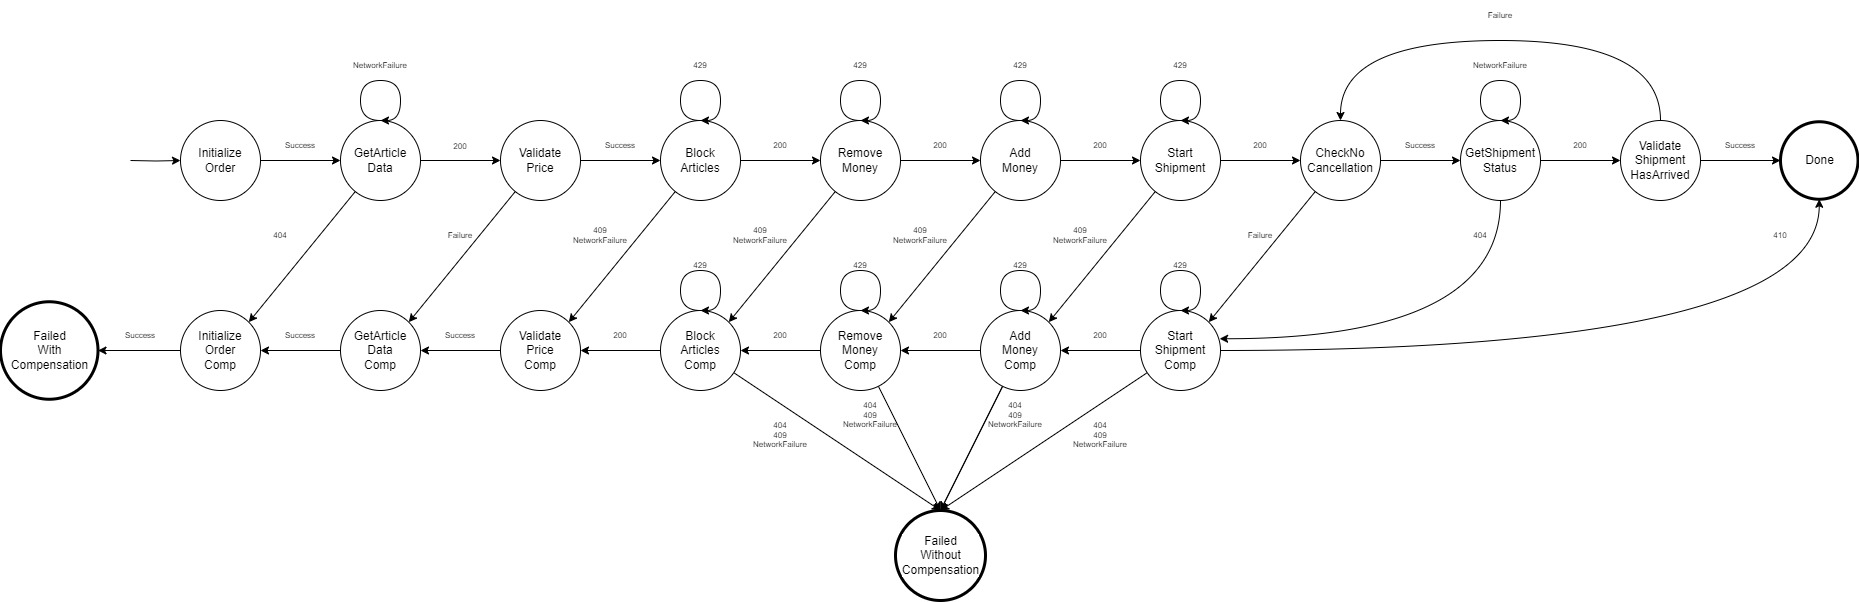
\includegraphics[width=\linewidth]{figures/ChapterVersuchsdurchführung/sm_basic_safe_retries.jpg}
	\caption{SmBasicSafeRetries}
	\label{fig:SmBasicSafeRetries}
\end{figure}
\FloatBarrier

\subsection{StateAnalysisResult}

\paragraph*{Testfall FinishOrders}
%TODO
\begin{center}
	\fontsize{9}{12}\selectfont
	\begin{longtable}[h]{|p{5cm}|p{1cm}|p{1cm}|p{1cm}|}
		\hline
		Messwert & S1 & S2 & S3 \\ \hline
		\endhead
		\caption{StateAnalysisResult SmBasicSafeRetries im Testfall FinishOrders}
		\label{tab:smbasicsaferetries_stateanalysisresult_finishorders}
		\endfoot
		successfull\-Percentage & 1.0 & 0.66 & 0.4 \\ \hline
		finished\-Percentage & 1.0 & 1.0 & 1.0 \\ \hline
		pending\-Percentage & 0.0 & 0.0 & 0.0 \\ \hline
		failedWithCompensation\-Percentage & 0 & 0.29 & 0.46 \\ \hline
		failedWithoutCompensation\-Percentage & 0.0 & 0.05 & 0.15 \\ \hline
		hasCorrectEndstate\-Percentage & 1.0 & 0.66 & 0.4 \\ \hline
		containsAllExpectedLogs\-Percentage & 1.0 & 0.66 & 0.4 \\ \hline
		isSuccessfullTestInstance\-Percentage & 1.0 & 0.66 & 0.4 \\ \hline
	\end{longtable}
\end{center}
\FloatBarrier

\paragraph*{Testfall CancelOrders}
%TODO
\begin{center}
	\fontsize{9}{12}\selectfont
	\begin{longtable}[h]{|p{5cm}|p{1cm}|p{1cm}|p{1cm}|}
		\hline
		Messwert & S1 & S2 & S3 \\ \hline
		\endhead
		\caption{StateAnalysisResult SmBasicSafeRetries im Testfall FinishOrders}
		\label{tab:smbasicsaferetries_stateanalysisresult_cancelorders}
		\endfoot
		successfull\-Percentage & 1.0 & 0.66 & 0.4 \\ \hline
		finished\-Percentage & 1.0 & 1.0 & 1.0 \\ \hline
		pending\-Percentage & 0.0 & 0.0 & 0.0 \\ \hline
		failedWithCompensation\-Percentage & 0 & 0.29 & 0.46 \\ \hline
		failedWithoutCompensation\-Percentage & 0.0 & 0.05 & 0.15 \\ \hline
		hasCorrectEndstate\-Percentage & 1.0 & 0.66 & 0.4 \\ \hline
		containsAllExpectedLogs\-Percentage & 1.0 & 0.66 & 0.4 \\ \hline
		isSuccessfullTestInstance\-Percentage & 1.0 & 0.66 & 0.4 \\ \hline
	\end{longtable}
\end{center}
\FloatBarrier

\section{Implementierung des SmBasicNetworkFailureUnlimitedRetries}

Der SmBasicNetworkFailureUnlimitedRetries baut auf das Konzept des vorherigen DEAs SmBasicSafeRetries auf. Es hat sich gezeigt, dass der Anteil der erfolgreichen Sagas erhöht werden kann, indem auf Netzwerkfehler per Forwardrecovery reagiert wird. Das Ziel dieses DEAs ist, den Anteil der vorzeitig abgebrochenen Sagas zu erhöhen. Dafür werden für die Ts \textit{BlockArticles}, \textit{RemoveMoney}, \textit{AddMoney} und \textit{StartShipment} sowie für die zugehörigen Cs ein Retry für Netzwerkfehler eingeführt. Es entsteht der DEA in \cref{fig:SmBasicNetworkfailureUnlimitedRetries}.

\begin{figure}[h!]
	\centering
	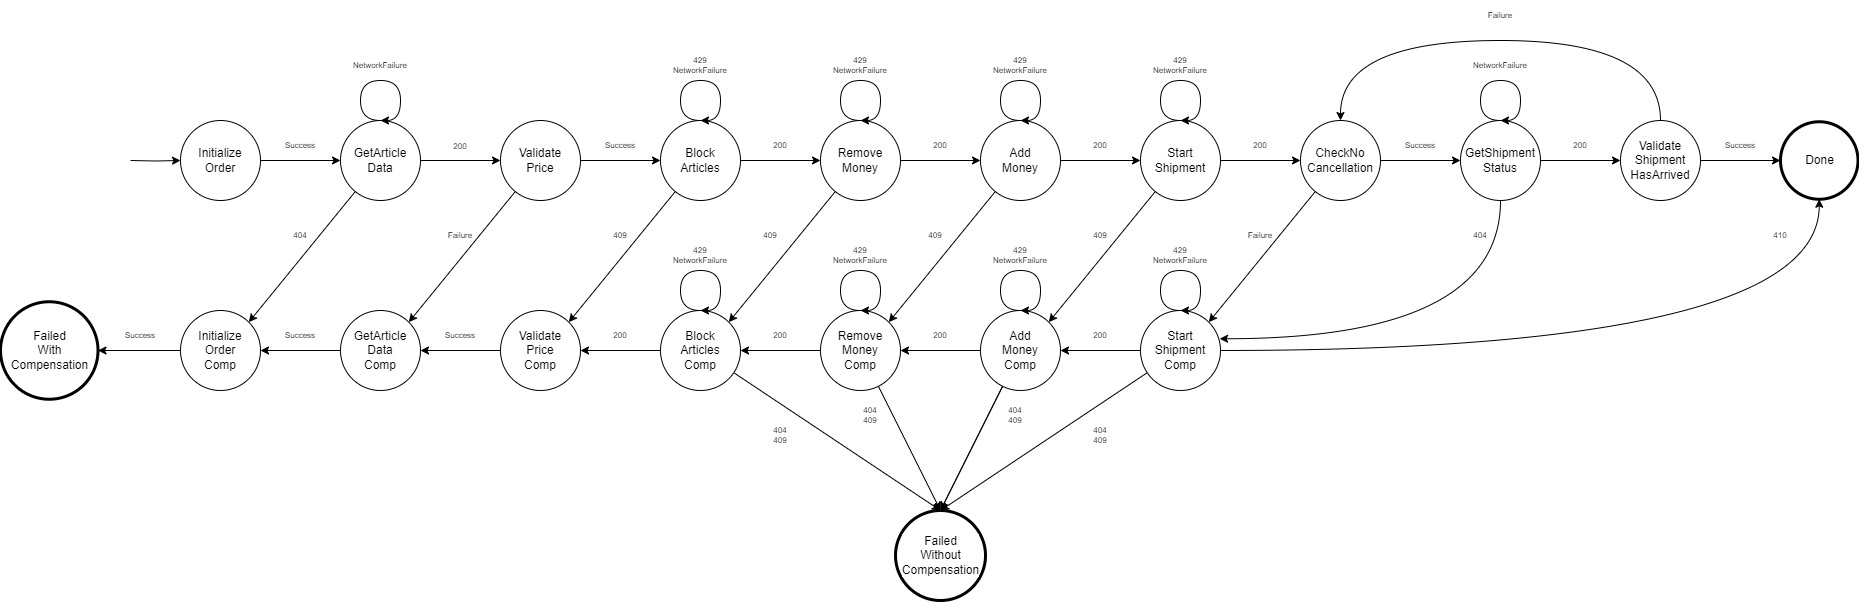
\includegraphics[width=\linewidth]{figures/ChapterVersuchsdurchführung/sm_basic_unlimited_retries.jpg}
	\caption{DEA für SmBasicNetworkfailureUnlimitedRetries}
	\label{fig:SmBasicNetworkfailureUnlimitedRetries}
\end{figure}
\FloatBarrier

\subsection{StateAnalysisResult}

Das StateAnalysisResult zeigt, dass das Einführen von Retries für transaktionelle Zustände dazu führt, dass der gewünschte Endzustand öfter erreicht wird. Testszenario 3 enthält in Testfall FinishOrders 90\% und in Testfall CancelOrders 74\% erfolgreiche Testinstanzen. Aus Sicht des Koordinators kann auf Netzwerkfehler mit einem Retry erfolgreich reagiert werden, um zum nächsten Zustand zu gelangen.

\paragraph*{Testfall FinishOrders}

\begin{center}
	\fontsize{9}{12}\selectfont
	\begin{longtable}[h]{|p{5cm}|p{1cm}|p{1cm}|p{1cm}|}
		\hline
		Messwert & S1 & S2 & S3 \\ \hline
		\endhead
		%\label{tab:smbasic_stateanalysisresult_finishorders}
		\endfoot
		successfull\-Percentage & 1.0 & 1.0 & 0.91 \\ \hline
		finished\-Percentage & 1.0 & 1.0 & 1.0 \\ \hline
		pending\-Percentage & 0.0 & 0.0 & 0.0 \\ \hline
		failedWithCompensation\-Percentage & 0.0 & 0.0 & 0.0 \\ \hline
		failedWithoutCompensation\-Percentage & 0.0 & 0.0 & 0.1 \\ \hline
		hasCorrectEndstate\-Percentage & 1.0 & 1.0 & 0.91 \\ \hline
		containsAllExpectedLogs\-Percentage & 1.0 & 1.0 & 0.91 \\ \hline
		isSuccessfullTestInstance\-Percentage & 1.0 & 1.0 & 0.91 \\ \hline
	\end{longtable}
\end{center}
\FloatBarrier

\paragraph*{Testfall CancelOrders}

\begin{center}
	\fontsize{9}{12}\selectfont
	\begin{longtable}[h]{|p{5cm}|p{1cm}|p{1cm}|p{1cm}|}
		\hline
		Messwert & S1 & S2 & S3 \\ \hline
		\endhead
		%\label{tab:smbasic_stateanalysisresult_finishorders}
		\endfoot
		successfull\-Percentage & 0.0 & 0.0 & 0.0 \\ \hline
		finished\-Percentage & 1.0 & 1.0 & 1.0 \\ \hline
		pending\-Percentage & 0.0 & 0.0 & 0.0 \\ \hline
		failedWithCompensation\-Percentage & 1.0 & 1.0 & 0.74 \\ \hline
		failedWithoutCompensation\-Percentage & 0.0 & 0.0 & 0.27 \\ \hline
		hasCorrectEndstate\-Percentage & 1.0 & 1.0 & 0.74 \\ \hline
		containsAllExpectedLogs\-Percentage & 1.0 & 1.0 & 0.74 \\ \hline
		isSuccessfullTestInstance\-Percentage & 1.0 & 1.0 & 0.74 \\ \hline
	\end{longtable}
\end{center}
\FloatBarrier

\subsection{TransactionAnalysisResult}
In \cref{tab:smbasic_stateanalysisresult} sind die TransactionAnalysisResults für beide Testfälle dargestellt. 

\begin{center}
	\fontsize{9}{12}\selectfont
	\begin{longtable}[h]{|p{5cm}|p{1cm}|p{1cm}|p{1cm}|}
		\hline
		& S1 & S2 & S3 \\ \hline
		\endhead
		%\label{tab:smbasic_stateanalysisresult}
		\endfoot
		FinishOrders & 1 & 1 & 0.67\\ \hline	
		CancelOrders & 1 & 1 & 0.36\\ \hline
	\end{longtable}
\end{center}
\FloatBarrier

Hier zeigt sich, dass im Vergleich zum SmBasicSafeRetries die Kennzahl \textit{consistentSagasPercentage} deutlich kleiner wird. Konsistenz des Systems hat sich durch die Einführung der Änderungen verringert. 

Aus Sicht des Koordinators ist der SmBasicNetworkFailureUnlimitedRetries erfolgreicher, der Vergleich von der Koordinator- und Teilnehmersicht zeigt jedoch, dass Transaktionen stattfinden, die der Koordinator nicht kennt. 

Es zeigt sich außerdem, dass diese Fehler lediglich in Testszenario 3 auftreten. Die fehlerverursachenden Transaktionen sind genau die, bei denen die Response auf dem Rückweg verloren geht. Der Koordinator interpretiert dies im Kontext dieses Zustandsautomaten als wiederholbar und führt die Transaktion erneut aus. Dadurch wird im entsprechenden Teilnehmerservice die Transaktion mehr als einmal ausgeführt. 

\section{Das Problem der Wiederholbarkeit}

In der Analyse des SmBasicNetworkFailureUnlimitedRetries hat sich gezeigt, dass die für die 4 Ts \textit{BlockArticles}, \textit{RemoveMoney}, \textit{AddMoney} und \textit{StartShipment} und ihre zugehörigen Cs eingeführten Retries zu inkonsistentem Verhalten in Testszenario 3 geführt haben. Das Problem besteht darin, dass lokale Transaktionen bei Wiederholung erneut ausgeführt werden. Dem Koordinator fehlt die Information, ob die lokale Transaktion im Fall eines Netzwerkfehlers bereits ausgeführt wurde oder nicht. 

\subsection{Implementierung von idempotentem Verhalten} 
Es wird ein idempotentes Verhalten benötigt, bei dem der Koordinator gefahrlos Aufrufe an den Teilnehmerservice wiederholen kann. Dazu muss jeder Teilnehmerservice die ausgeführten Transaktionen mit einer zugehörigen RequestId speichern. Taucht ein Request mit einer bereits verwendeten RequestId auf, wird der Request nicht erneut bearbeitet, sondern eine Response mit dem Statuscode 208 zurückgegeben. Damit erhält der Aufrufer die Information, dass der Request bereits erfolgreich verarbeitet wurde. 

Um idempotentes Verhalten zu implementieren, muss ein Service jeden erfolgreichen Request mit der zugehörigen RequestId abspeichern. Diese Information werden in einer Tabelle persistiert. Die Prüfung, ob ein Request prozessiert werden kann, ist eine Fallunterscheidung. Wenn ein Eintrag in der Idempotenztabelle existiert, der in RequestId und Transaktion übereinstimmt, wird der Request mit 208 abgelehnt. Existiert kein solcher Datensatz, kann die Transaktion prozessiert werden.

\subsection{Idempotente DEAs}
Die drei DEAs SmBasic, SmBasicSafeRetries und SmBasicNetworkFailureUnlimitedRetries verwenden die nicht-idempotenten Implementierungen der Teilnehmerservices. Damit nicht-idempotente und idempotente DEAs verglichen werden können, sind alle Teilnehmerservices hinsichtlich Idempotenz konfigurierbar. Die Fallunterscheidung, die bereits ausgeführte Transaktionen ablehnt, wird bei einer nicht-idempotenten Konfiguration des Services übersprungen. Die folgenden zwei DEAs verwenden eine idempotente Konfiguration. 

\section{Implementierung des SmIdempotencyBackwardRecovery}
Der erste idempotente DEA wird als SmIdempotencyBackwardRecovery bezeichnet. Im Falle eines Netzwerkfehlers bei einem T wird ein Übergang zum entsprechenden C eingeführt; die Saga wird also versucht zurückzurollen, unabhängig ob das T ausgeführt wurde oder nicht. In \cref{fig:fig_sm_idempotency_backward_recovery_testcase2} ist der Fall abgebildet, dass ein T einen Netzwerkfehler verursacht ohne eine Zustandsänderung im Teilnehmerservice zu bewirken. \Cref{fig:fig_sm_idempotency_backward_recovery_testcase3} zeigt den Ablauf im Fall eines Netzwerkfehlers mit Zustandsänderung. 

\begin{figure}[h!]
	\centering
	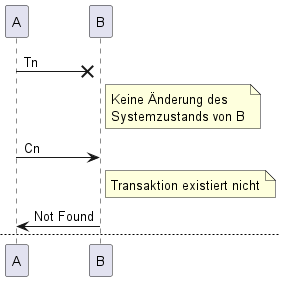
\includegraphics[width=0.3\linewidth]{figures/ChapterVersuchsdurchführung/SmIdempotencyBackwardRecovery-0.png}
	\caption{Sequenzdiagramm für Idempotentes Verhalten bei wiederholten Anfragen in Szenario 3}
	\label{fig:fig_sm_idempotency_backward_recovery_testcase2}
\end{figure}

\FloatBarrier
\begin{figure}[h!]
	\centering
	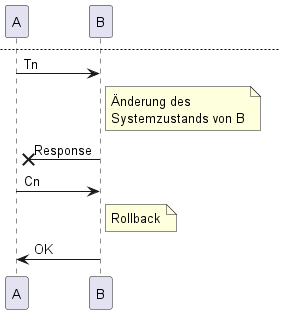
\includegraphics[width=0.3\linewidth]{figures/ChapterVersuchsdurchführung/SmIdempotencyBackwardRecovery-1.png}
	\caption{Sequenzdiagramm für Idempotentes Verhalten bei wiederholten Anfragen in Szenario 3}
	\label{fig:fig_sm_idempotency_backward_recovery_testcase3}
\end{figure}
\FloatBarrier

Solche Fehler treten jedoch auch bei den Cs auf. Deshalb müssen diese auch addressiert werden. Bei Fehlschlagen eines Cs könnte in den Zustand FailedWithoutCompensation gewechselt werden. Dies soll jedoch verhindert werden. Da die Teilnehmerservices idempotentes Verhalten unterstützen, können Cs wiederholt werden, bis ein eindeutiges Ergebnis vorliegt. In folgenden Fällen kann ein Übergang zum nächsten C eingeführt werden:
\begin{itemize}
	\item 200: Die Transaktion wurde erfolgreich kompensiert
	\item 208: Die Transaktion wurde in einem vorherigen Schritt bereits erfolgreich kompensiert
	\item 404: Die Transaktion ist nicht bekannt und muss nicht kompensiert werden
\end{itemize}

Im Falle eines Konflikts (409) muss jedoch weiterhin auf den Zustand FailedWithoutCompensation gewechselt werden.

Der resultierende Zustandsautomat ist in \cref{fig:fig_sm_idempotency_backward_recovery} abgebildet.

\begin{figure}[h!]
	\centering
	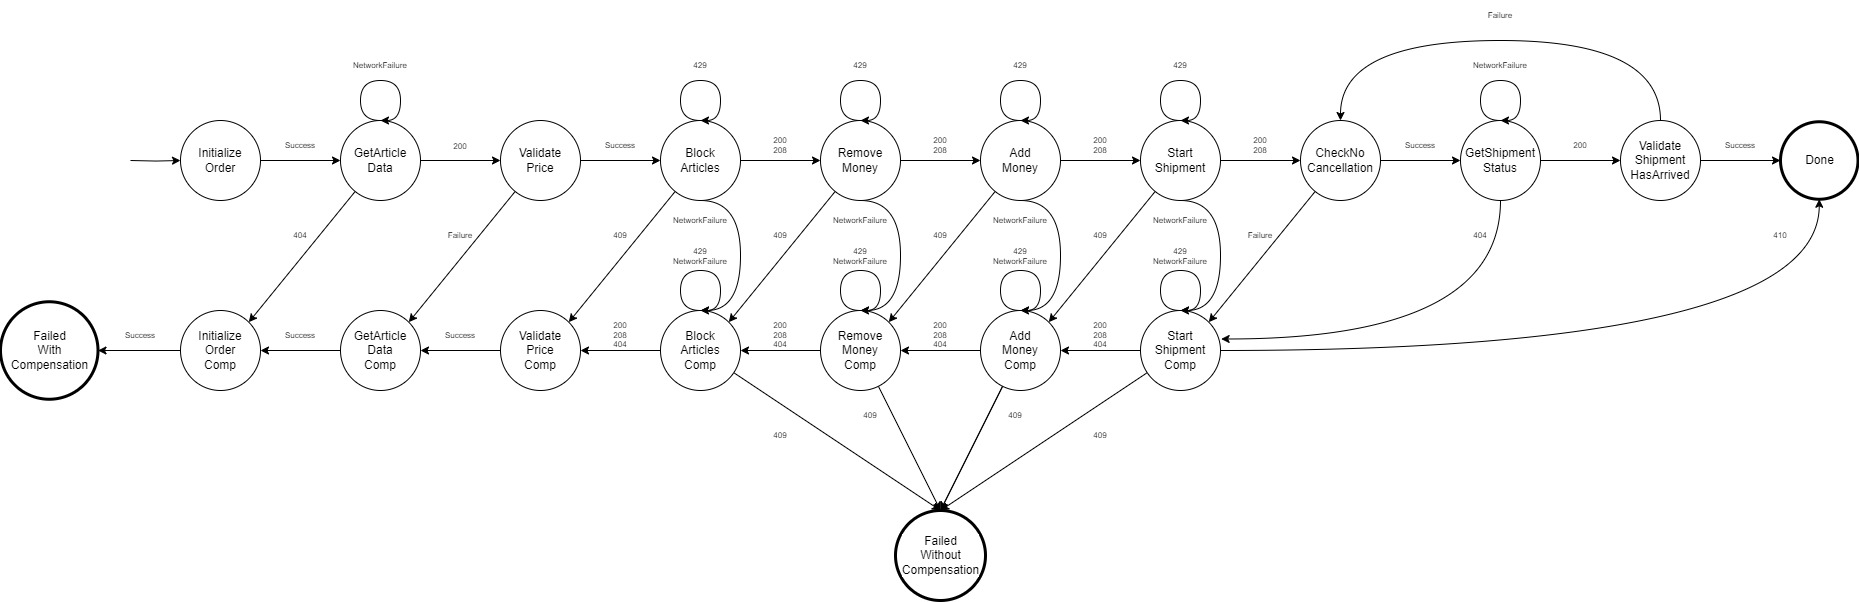
\includegraphics[width=\linewidth]{figures/ChapterVersuchsdurchführung/sm_idempotency_backward_recovery.jpg}
	\caption{DEA für SmIdempotencyBackwardRecovery}
	\label{fig:fig_sm_idempotency_backward_recovery}
\end{figure}
\FloatBarrier

\subsection{StateAnalysisResult}

Das StateAnalysisResult zeigt einen hohen Anteil an vorzeitig abgebrochenen Sagas. Das ist mit dem Konzept der Backwardrecovery begründet. Lediglich Testszenario 1 liefert in beiden Testfällen eine Erfolgsrate von 100\%.

\paragraph*{Testfall FinishOrders}

\begin{center}
	\fontsize{9}{12}\selectfont
	\begin{longtable}[h]{|p{5cm}|p{1cm}|p{1cm}|p{1cm}|}
		\hline
		Messwert & S1 & S2 & S3 \\ \hline
		\endhead
		%\label{tab:smbasic_stateanalysisresult_finishorders}
		\endfoot
		successfull\-Percentage & 1.0 & 0.63 & 0.44 \\ \hline
		finished\-Percentage & 1.0 & 1.0 & 1.0 \\ \hline
		pending\-Percentage & 0.0 & 0.0 & 0.0 \\ \hline
		failedWithCompensation\-Percentage & 0.0 & 0.38 & 0.57 \\ \hline
		failedWithoutCompensation\-Percentage & 0.0 & 0.0 & 0.0 \\ \hline
		hasCorrectEndstate\-Percentage & 1.0 & 0.63 & 0.39 \\ \hline
		containsAllExpectedLogs\-Percentage & 1.0 & 0.63 & 0.44 \\ \hline
		isSuccessfullTestInstance\-Percentage & 1.0 & 0.63 & 0.44 \\ \hline
	\end{longtable}
\end{center}
\FloatBarrier

\paragraph*{Testfall CancelOrders}

\begin{center}
	\fontsize{9}{12}\selectfont
	\begin{longtable}[h]{|p{5cm}|p{1cm}|p{1cm}|p{1cm}|}
		\hline
		Messwert & S1 & S2 & S3 \\ \hline
		\endhead
		%\label{tab:smbasic_stateanalysisresult_finishorders}
		\endfoot
		successfull\-Percentage & 0.0 & 0.0 & 0.0 \\ \hline
		finished\-Percentage & 1.0 & 1.0 & 1.0 \\ \hline
		pending\-Percentage & 0.0 & 0.0 & 0.0 \\ \hline
		failedWithCompensation\-Percentage & 1.0 & 1.0 & 1.0 \\ \hline
		failedWithoutCompensation\-Percentage & 0.0 & 0.0 & 0.0 \\ \hline
		hasCorrectEndstate\-Percentage & 1.0 & 1.0 & 1.0 \\ \hline
		containsAllExpectedLogs\-Percentage & 1.0 & 0.68 & 0.44 \\ \hline
		isSuccessfullTestInstance\-Percentage & 1.0 & 0.68 & 0.44 \\ \hline
	\end{longtable}
\end{center}
\FloatBarrier

\subsection{TransactionAnalysisResult}
In \cref{tab:smbasic_stateanalysisresult} sind die TransactionAnalysisResults für beide Testfälle dargestellt. Überraschend ist hier der niedrige Anteil an konsistenten Sagas in Testszenario 2 und 3. 

\begin{center}
	\fontsize{9}{12}\selectfont
	\begin{longtable}[h]{|p{5cm}|p{1cm}|p{1cm}|p{1cm}|}
		\hline
		& S1 & S2 & S3 \\ \hline
		\endhead
		%\label{tab:smbasic_stateanalysisresult}
		\endfoot
		FinishOrders & 1 & 1 & 0.74\\ \hline	
		CancelOrders & 1 & 1 & 0.74\\ \hline
	\end{longtable}
\end{center}
\FloatBarrier

Die Ursache dafür liegt in der Berechnung der Kennzahl sowie dem Aufbau des Zustandsautomaten. Für die Berechnung der Kennzahl werden die Differenzen der jeweiligen Transaktionen nach Koordinator- und Teilnehmersicht gebildet. Nur wenn diese für jedes T und jedes C übereinstimmen fließt das Ergebnis als erfolgreich in die Kennzahl ein. 

Konkret soll nun diese Messungenauigkeit betrachtet werden. Wird die Anzahl einer Transaktion in Koordinatorsicht berechnet, wird das Transaktionslog verwendet. Dabei soll das in \cref{fig:fig} dargestellte Transaktionslog verwendet werden. 

Das Log zeigt eine Saga, die aufgrund eines Netzwerkfehlers im Zustand \textit{StartShipment} zur Kompensierung wechselt. Zur Berechnung für die Kennzahl \textit{consistentSagasPercentage} wird auch die Anzahl der Transaktionen mit dem Zustand \textit{StartShipment} und dem Ergebnis \textit{StartShipment200} oder \textit{StartShipment208} berechnet. Für den SmIdempotencyBackwardRecovery bedeutet ein Netzwerkfehler in den kritischen Ts, dass das dazugehörige C die Änderungen kompensiert oder fortfährt, falls der Netzwerkfehler keine Zustandsänderungen bewirkt hat. Das Zählen der Transaktionen mit dem Zustand \textit{StartShipment} und dem Ergebnis \textit{StartShipment200} oder \textit{StartShipment208} ist für diesen DEA also keine korrekte Berechnung, um Konsistenz zu messen.

\begin{center}
	\fontsize{9}{12}\selectfont
	\begin{longtable}[h]{|p{4.5cm}|p{6.5cm}|}
		\hline
		Zustand & Ergebnis \\* \hline
		\endhead
		\hline
		\caption{Transaktionslog für Saga im Testfall CancelOrders und Testszenario 2}
		\label{tab:transaktionslog_ts2_cancelorders_smbasic}
		\endfoot
		InitializeOrder & InitializeSagaSuccess \\* \hline
		GetArticleData & GetProductData200 \\* \hline
		ValidatePrice & ValidatePriceSuccess \\* \hline
		BlockArticles & BlockArticles200 \\* \hline
		RemoveMoney & RemoveMoney200 \\* \hline
		AddMoney & AddMoney200 \\* \hline
		\rowcolor{Gray}
		StartShipment & StartShipmentNetworkFailure \\* \hline
		StartShipmentCompensation & StartShipmentCompensationNetworkFailure \\* \hline
		\rowcolor{Gray}
		StartShipmentCompensation & StartShipmentCompensation208 \\* \hline
		AddMoneyCompensation & AddMoneyCompensation200 \\* \hline
		RemoveMoneyCompensation & RemoveMoneyCompensation200 \\* \hline
		BlockArticlesCompensation & BlockArticlesCompensation200 \\* \hline
		ValidatePriceCompensation & ValidatePriceCompensationSuccess \\* \hline
		GetArticleDataCompensation & GetProductDataCompensationSuccess \\* \hline
		InitializeOrderCompensation & InitializeSagaCompensationSuccess \\* \hline
	\end{longtable}
\end{center}
\FloatBarrier

\subsection{Alternative Sicherstellung der Konsistenz}
Damit der Zustandsautomat trotz dieser verfälschten Messung bewertet werden kann, wird eine Alternative benötigt. Um eine Aussage über die Konsistenz zu treffen, kann der Inhalt der eigentlichen Tabellen der Services verwendet werden. 

\paragraph*{Alternative Konsistenzdefinition}\label{par:consistency_definition_alt}
Als Konsistenzkriterien dienen folgende Annahmen:
\begin{itemize}
	\item Die Summe des Geldes im System bleibt gleich.
	\item Die Summer aller Artikel im System bleibt gleich.
\end{itemize}

\paragraph*{Einordnung dieser Definition}
Diese Vorgehensweise kann entscheiden, ob das System nach den definierten Regeln im konsistenten Zustand bleibt oder ob eine Transaktion das System in einen inkonsistenten Zustand überführt hat. Dies ist eine binäre Messung, über die Qualität der Konsistenz kann im vorliegenden System, unter Verwendung dieses Zustandsautomaten und unter Verwendung des aktuellen Versuchsaufbaus keine Aussage getroffen werden. 

Nach den genannten Annahmen ist das System auch konsistent, wenn zwei parallele Sagas fehlschlagen und eine Saga \textit{AddMoney} und die andere Saga \textit{RemoveMoney} jeweils doppelt mit dem (zufällig) identischen Betrag ausführen. Die Menge des Geldes im System bleibt trotz Auftreten eines solchen hypothetischen Bugs konsistent. 

Diese Erläuterung soll verdeutlichen, dass die sehr vage Definition von Konsistenz mit Vorsicht verwendet werden sollte. Für diesen Automaten soll dies jedoch ausreichen. 

\paragraph{Messung}
Die Messung erfolgt manuell. Die Summe des im System befindlichen Geldes wird vor Ausführung der Tests gemessen. Dabei ist jedes Konto mit einem Startcredit von 15000.00 initialisiert. Tritt ein Konsistenzfehler bei Verwendung der BankServices auf, so wird dies in diesem Statement deutlich, wenn sich die zwei Werte \textit{expectedCreditSum} und \textit{actualCreditSum} unterscheiden.

\begin{lstlisting}[language=SQL, breaklines=true, tabsize=2, showstringspaces=false, frame=single, numbers=left, basicstyle=\small] 
select case when 
	15000.00 * cast(
		(select count(*) from bank1user) + 
		(select count(*) from bank2user) as float) 
	= cast(
		(select sum(credit) from bank1credit) + 
		(select sum(credit) from bank2credit) as float)
	then 1 else 0 end as mightBeConsistent;
\end{lstlisting}\label{}

Die Anzahl der Artikel wird mit einem vergleichbaren Statement auf Konsistenz überprüft. Die Summe der Artikel wird über die drei Tabellen des StockServices gezählt. Ändert sich diese Zahl nach Ausführung der Tests, ist ein Konsistenzfehler aufgetreten.

\begin{lstlisting}[language=SQL, breaklines=true, tabsize=2, showstringspaces=false, frame=single, numbers=left, basicstyle=\small] 
select case when 
	(select 15000 * count(*) from articlestock as expectedarticlesum) 
	= 
	(select sum(amount) as amount from (
		select articleid as articleid, amount as amount from articlestock
		union
		select articleid, sum(amount) as amount from blockedarticles group by articleid
		union
		select articleidfk as articleid, sum(amount) as amount from shippedarticles group by articleidfk) as actualarticlesum
	)
	then 1 else 0 end as mightBeConsistent;
\end{lstlisting}\label{}

Ändert sich in beiden Tests die Summe nicht, ist laut \cref{par:consistency_definition_alt} die notwendige Bedingung für Konsistenz erreicht. Das Gesamtergebnis berechnet sich durch folgendes Statement:
\begin{lstlisting}[language=SQL, breaklines=true, tabsize=2, showstringspaces=false, frame=single, numbers=left, basicstyle=\small] 
with moneyMightBeConsistent as (
	select case when 
		(select 15000 * count(*) from articlestock as expectedarticlesum) 
		= 
		(select sum(amount) as amount from (
		select articleid as articleid, amount as amount from articlestock
		union
		select articleid, sum(amount) as amount from blockedarticles group by articleid
		union
		select articleidfk as articleid, sum(amount) as amount from shippedarticles group by articleidfk) as actualarticlesum
	)
	then 1 else 0 end as mightBeConsistent),
articleMightBeConsistent as (
	select case when 
		15000.00 * cast(
			(select count(*) from bank1user) + 
			(select count(*) from bank2user) as float) 
		= cast(
			(select sum(credit) from bank1credit) + 
			(select sum(credit) from bank2credit) as float)
		then 1 else 0 end as mightBeConsistent) 
select moneyMightBeConsistent.mightBeConsistent as moneyMightBeConsistent,
	articleMightBeConsistent.mightBeConsistent as articleMightBeConsistent,
	case when 
		moneyMightBeConsistent.mightBeConsistent 
		= 
		articleMightBeConsistent.mightBeConsistent 
	then 1 else 0 end as mightBeConsistent
from moneyMightBeConsistent, articleMightBeConsistent;
\end{lstlisting}\label{}

\paragraph*{Ergebnis}
Die Messung ist für beide 

\begin{center}
	\fontsize{9}{12}\selectfont
	\begin{longtable}[h]{|p{4cm}|p{1cm}|p{1cm}|p{1cm}|}
		\hline
		 & S1 & S2 & S3 \\ \hline
		\endhead
		\caption{Messwert \textit{altConsistentSagasPercentage} für SmIdempotencyBackwardRecovery}
		\label{tab:smbasic_stateanalysisresult}
		\endfoot
		moneyMightBeConsistent & 1 & 1 & 1 \\ \hline	
		articleMightBeConsistent & 1 & 1 & 1 \\ \hline
		mightBeConsistent & 1 & 1 & 1 \\ \hline
	\end{longtable}
\end{center}
\FloatBarrier


\section{Implementierung SmIdempotencyForwardRecovery}
Die Auswertung der Ergebnisse des SmIdempotencyBackwardRecovery hat gezeigt, dass die Strategie der BackwardRecovery Konsistenz gewährleisten kann. Dabei trat jedoch erneut das Problem des vorzeitigen Abbruchs auf. Das erste Vorkommen eines Netzwerkfehlers innerhalb eines Ts führte zur Kompensierung. Der nächste zu implementierende Zustandsautomat verfolgt zwei Ziele: eine möglichst hohe Erfolgsrate sowie Konsistenz. Mittels ForwardRecovery kann eine Weiterführung der Saga erzwungen werden. Abgebrochen wird lediglich in Zuständen, bei denen ein Ergebnis auftritt, das nicht behebbar ist. 

Für Ts ist lediglich ein Ergebnis wie 409 unbehebbar und es wird zum vorherigen C gewechselt. Für Netzwerkfehler werden Retries eingeführt. Aufgrund der Idempotenz der Teilnehmerservices ist dies problemlos möglich. Nur bei einem eindeutigen Ergebnis wird fortgefahren (200, 208) oder abgebrochen (409). 

Der resultierende Zustandsautomat SmIdempotencyForwardRecovery ist in \cref{fig:SmIdempotencyForwardRecovery} abgebildet.


\begin{figure}[h!]
	\centering
	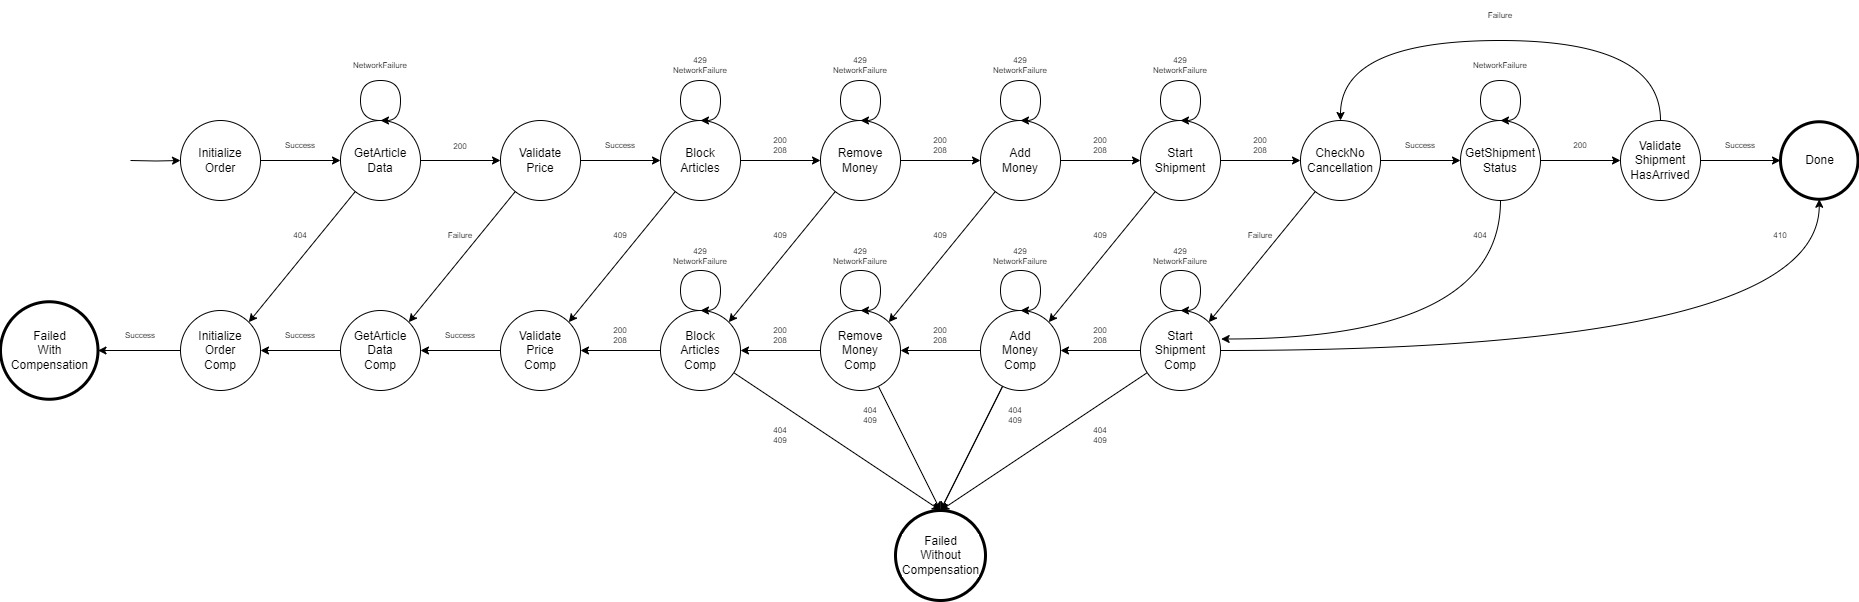
\includegraphics[width=\linewidth]{figures/ChapterVersuchsdurchführung/sm_idempotency_forward_recovery.jpg}
	\caption{DEA für SmIdempotencyForwardRecovery}
	\label{fig:SmIdempotencyForwardRecovery}
\end{figure}
\FloatBarrier

\subsection{StateAnalysisResult}

Das StateAnalysisResult zeigt, dass unabhängig vom Testfall und Testszenario alle Sagas im erwarteten Endzustand münden. 

\paragraph*{Testfall FinishOrders}

\begin{center}
	\fontsize{9}{12}\selectfont
	\begin{longtable}[h]{|p{5cm}|p{1cm}|p{1cm}|p{1cm}|}
		\hline
		Messwert & S1 & S2 & S3 \\ \hline
		\endhead
		%\label{tab:smbasic_stateanalysisresult_finishorders}
		\endfoot
		successfull\-Percentage & 1.0 & 1.0 & 0.91 \\ \hline
		finished\-Percentage & 1.0 & 1.0 & 1.0 \\ \hline
		pending\-Percentage & 0.0 & 0.0 & 0.0 \\ \hline
		failedWithCompensation\-Percentage & 0.0 & 0.0 & 0.0 \\ \hline
		failedWithoutCompensation\-Percentage & 0.0 & 0.0 & 0.1 \\ \hline
		hasCorrectEndstate\-Percentage & 1.0 & 1.0 & 1.0 \\ \hline
		containsAllExpectedLogs\-Percentage & 1.0 & 1.0 & 1.0 \\ \hline
		isSuccessfullTestInstance\-Percentage & 1.0 & 1.0 & 1.0 \\ \hline
	\end{longtable}
\end{center}
\FloatBarrier

\paragraph*{Testfall CancelOrders}

\begin{center}
	\fontsize{9}{12}\selectfont
	\begin{longtable}[h]{|p{5cm}|p{1cm}|p{1cm}|p{1cm}|}
		\hline
		Messwert & S1 & S2 & S3 \\ \hline
		\endhead
		%\label{tab:smbasic_stateanalysisresult_finishorders}
		\endfoot
		successfull\-Percentage & 0.0 & 0.0 & 0.0 \\ \hline
		finished\-Percentage & 1.0 & 1.0 & 1.0 \\ \hline
		pending\-Percentage & 0.0 & 0.0 & 0.0 \\ \hline
		failedWithCompensation\-Percentage & 1.0 & 1.0 & 1.0 \\ \hline
		failedWithoutCompensation\-Percentage & 0.0 & 0.0 & 0.0 \\ \hline
		hasCorrectEndstate\-Percentage & 1.0 & 1.0 & 1.0 \\ \hline
		containsAllExpectedLogs\-Percentage & 1.0 & 1.0 & 1.0 \\ \hline
		isSuccessfullTestInstance\-Percentage & 1.0 & 1.0 & 1.0 \\ \hline
	\end{longtable}
\end{center}
\FloatBarrier

\subsection{TransactionAnalysisResult}
In \cref{tab:smbasic_stateanalysisresult} sind die TransactionAnalysisResults für beide Testfälle dargestellt. Es ist erkennbar, dass die Konsistenz in beiden Testfällen für alle Testszenarios eingehalten wird. 

\begin{center}
	\fontsize{9}{12}\selectfont
	\begin{longtable}[h]{|p{2cm}|p{1cm}|p{1cm}|p{1cm}|}
		\hline
		 & S1 & S2 & S3 \\ \hline
		\endhead
		%\label{tab:smbasic_stateanalysisresult}
		\endfoot
		FinishOrders & 1 & 1 & 1 \\ \hline	
		CancelOrders & 1 & 1 & 1 \\ \hline
	\end{longtable}
\end{center}
\FloatBarrier

\section{Laufzeitanalyse}

Das primäre Werkzeug der Optimierung der Zustandsautomaten war die Einführung von Retries. Es ist zu erwarten, dass die Einführung von Retries die Laufzeit verlängert. Im Folgenden sind die Ergebnisse der Laufzeitanalyse per Boxplot dargestellt. Als Visualisierung wird ein modifizierter Boxplot verwendet. In jedem Diagramm sind das obere und untere Quartil, der Median, das Maximum und Minimum sowie Ausreißer ablesbar. Jeder Boxplot stellt die Werte eines DEAs dar. Aus Gründen der Übersicht wurden die langen Bezeichnungen der Zustandsautomaten durch folgende Nummerierung ersetzt:

\begin{center}
	\begin{tabular}[h]{|p{8cm}|p{3cm}|}
		\hline
		Zustandsautomat & Nummerierung \\ \hline
		SmBasic & 1 \\ \hline
		SmBasicSafeRetries & 2 \\ \hline
		SmBasicNetworkFailureUnlimitedRetries & 3 \\ \hline
		SmIdempotencyBackwardRecovery & 4 \\ \hline		
		SmIdempotencyForwardRecovers & 5 \\ \hline
	\end{tabular}
\end{center}
\FloatBarrier

Es ist erkennbar, dass die Laufzeit für alle Automaten sehr nah beieinander liegt. Da im ersten Szenario keine Netzwerkfehler auftauchen, sind die Werte sehr wenig gestreut. Die Ausreißer sind ebenfalls erkennbar.

\subsection{Testszenario1}

\begin{figure}[!htbp]
\begin{minipage}{.45\textwidth}
	
\begin{tikzpicture}
	\begin{axis} [
		boxplot/draw direction=y,
		%area legend,
		height=8.0cm, width=\linewidth,
		xmin=0,xmax=6,xtick={1,2,3,4,5},
		xtick style = {draw=none}, % Hide tick line
		enlarge x limits,
		ymin=0, ymax=100, ytick={0,20,...,100},
		ylabel = {Laufzeit [s]},
		ymajorgrids,
		ytick style = {draw=none}, % Hide tick line
		enlarge y limits,
		every axis plot/.append style={fill,fill opacity=0.5},
		every boxplot/.style={mark=x,every mark/.append style={mark size=1.0pt}}
		]
		% 
		\addplot+ [boxplot prepared={upper quartile=54.29, lower quartile=42.51, upper whisker=71.96, lower whisker=24.84, median=50.05, draw position=1}, ] coordinates {(1, 11.2)(1, 16.85)(1, 17.92)(1, 18.43)(1, 18.52)(1, 18.85)(1, 19.1)(1, 19.35)(1, 19.39)(1, 19.47)(1, 20.03)(1, 20.16)(1, 20.71)(1, 21.52)(1, 21.63)(1, 22.54)(1, 22.74)(1, 23.11)(1, 23.18)(1, 23.27)(1, 23.45)(1, 23.7)(1, 24.12)(1, 24.38)};
		\addplot+ [boxplot prepared={upper quartile=58.16, lower quartile=46.64, upper whisker=75.44, lower whisker=29.36, median=52.17, draw position=2}, ] coordinates {};
		\addplot+ [boxplot prepared={upper quartile=58.33, lower quartile=45.94, upper whisker=76.92, lower whisker=27.36, median=50.05, draw position=3}, ] coordinates {(3, 80.85)(3, 83.43)};
		\addplot+ [boxplot prepared={upper quartile=59.87, lower quartile=46.49, upper whisker=79.94, lower whisker=26.42, median=50.64, draw position=4}, ] coordinates {};
		\addplot+ [boxplot prepared={upper quartile=58.71, lower quartile=50.14, upper whisker=71.57, lower whisker=37.29, median=53.97, draw position=5}, ] coordinates {};
		
	\end{axis}
\end{tikzpicture}
	\caption{Boxplot FinishOrders in Szenario 1}
	\label{fig:boxplot_finishorders_scenario1}
\end{minipage}\hspace{\fill}%
\begin{minipage}{.45\textwidth}
	\begin{tikzpicture}
	\begin{axis} [
		boxplot/draw direction=y,
		%area legend,
		height=8.0cm, width=\linewidth,
		xmin=0,xmax=6,xtick={1,2,3,4,5},
		xtick style = {draw=none}, % Hide tick line
		enlarge x limits,
		ymin=0, ymax=140, ytick={0,20,...,140},
		ylabel = {Laufzeit [s]},
		ymajorgrids,
		ytick style = {draw=none}, % Hide tick line
		enlarge y limits,
		every axis plot/.append style={fill,fill opacity=0.5},
		every boxplot/.style={mark=x,every mark/.append style={mark size=1.0pt}}
		]
		% 
		\addplot+ [boxplot prepared={upper quartile=82.18, lower quartile=63.92, upper whisker=109.57, lower whisker=36.53, median=71.92, draw position=1}, ] coordinates {(1, 13.27)(1, 13.79)(1, 18.29)(1, 18.84)(1, 19.14)(1, 19.72)(1, 20.44)(1, 20.47)(1, 21.37)(1, 23.87)(1, 24.39)(1, 25.28)(1, 25.9)(1, 26.26)(1, 27.92)};
		\addplot+ [boxplot prepared={upper quartile=79.96, lower quartile=62.82, upper whisker=105.67, lower whisker=37.11, median=66.71, draw position=2}, ] coordinates {(2, 109.77)(2, 110.53)(2, 111.07)(2, 112.63)};
		\addplot+ [boxplot prepared={upper quartile=82.83, lower quartile=66.65, upper whisker=107.1, lower whisker=42.38, median=71.76, draw position=3}, ] coordinates {(3, 109.05)(3, 112.61)};
		\addplot+ [boxplot prepared={upper quartile=71.11, lower quartile=61.99, upper whisker=84.79, lower whisker=48.31, median=67.06, draw position=4}, ] coordinates {(4, 45.01)(4, 45.23)(4, 46.59)(4, 47.09)(4, 86.45)(4, 86.52)(4, 87.74)(4, 90.29)(4, 93.78)(4, 94.11)};
		\addplot+ [boxplot prepared={upper quartile=86.44, lower quartile=64.11, upper whisker=119.94, lower whisker=30.62, median=77.08, draw position=5}, ] coordinates {(5, 121.27)(5, 128.37)};
		
		
	\end{axis}
\end{tikzpicture}
	\caption{Boxplot CancelOrders in Szenario 1}
	\label{fig:boxplot_cancelorders_scenario1}
\end{minipage}
\end{figure}
\FloatBarrier

\subsection{Testszenario2}

\begin{figure}[!htbp]
\begin{minipage}{.45\textwidth}
	\begin{tikzpicture}
	\begin{axis} [
		boxplot/draw direction=y,
		%area legend,
		height=8.0cm, width=\linewidth,
		xmin=0,xmax=6,xtick={1,2,3,4,5},
		xtick style = {draw=none}, % Hide tick line
		enlarge x limits,
		ymin=0, ymax=160, ytick={0,20,...,160},
		ylabel = {Laufzeit [s]},
		ymajorgrids,
		ytick style = {draw=none}, % Hide tick line
		enlarge y limits,
		every axis plot/.append style={fill,fill opacity=0.5},
		every boxplot/.style={mark=x,every mark/.append style={mark size=1.0pt}}
		]
		% 
		\addplot+ [boxplot prepared={upper quartile=52.08, lower quartile=5.19, upper whisker=122.42, lower whisker=0.0, median=22.41, draw position=1}, ] coordinates {};
		\addplot+ [boxplot prepared={upper quartile=56.52, lower quartile=23.91, upper whisker=105.44, lower whisker=0.0, median=47.41, draw position=2}, ] coordinates {};
		\addplot+ [boxplot prepared={upper quartile=62.87, lower quartile=52.21, upper whisker=78.86, lower whisker=36.22, median=56.77, draw position=3}, ] coordinates {(3, 79.24)(3, 80.46)(3, 84.34)(3, 87.85)(3, 89.73)(3, 90.99)(3, 91.46)(3, 94.78)(3, 96.65)(3, 97.25)(3, 97.69)(3, 101.48)(3, 111.56)};
		\addplot+ [boxplot prepared={upper quartile=51.25, lower quartile=29.41, upper whisker=84.01, lower whisker=0.0, median=41.6, draw position=4}, ] coordinates {(4, 87.31)};
		\addplot+ [boxplot prepared={upper quartile=61.88, lower quartile=46.44, upper whisker=85.04, lower whisker=23.28, median=53.52, draw position=5}, ] coordinates {(5, 86.24)(5, 87.15)(5, 90.83)(5, 101.85)(5, 106.66)(5, 115.02)};
		
	\end{axis}
\end{tikzpicture}
	\caption{Boxplot FinishOrders in Szenario 2}
	\label{fig:boxplot_finishorders_scenario2}
\end{minipage}\hspace{\fill}%
\begin{minipage}{.45\textwidth}
	\begin{tikzpicture}
	\begin{axis} [
	 	boxplot/draw direction=y,
	 	%area legend,
		height=8.0cm, width=\linewidth,
	 	xmin=0,xmax=6,xtick={1,2,3,4,5},
	 	xtick style = {draw=none}, % Hide tick line
	 	enlarge x limits,
	 	ymin=0, ymax=160, ytick={0,20,...,160},
	 	ylabel = {Laufzeit [s]},
	 	ymajorgrids,
	 	ytick style = {draw=none}, % Hide tick line
	 	enlarge y limits,
	 	every axis plot/.append style={fill,fill opacity=0.5},
	 	every boxplot/.style={mark=x,every mark/.append style={mark size=1.0pt}}
	 	]
	 	% 
		\addplot+ [boxplot prepared={upper quartile=60.61, lower quartile=3.33, upper whisker=146.53, lower whisker=0.0, median=17.97, draw position=1}, ] coordinates {};
		\addplot+ [boxplot prepared={upper quartile=67.01, lower quartile=15.64, upper whisker=144.07, lower whisker=0.0, median=60.54, draw position=2}, ] coordinates {};
		\addplot+ [boxplot prepared={upper quartile=86.73, lower quartile=67.71, upper whisker=115.26, lower whisker=39.18, median=76.62, draw position=3}, ] coordinates {(3, 116.89)(3, 119.51)(3, 127.43)};
		\addplot+ [boxplot prepared={upper quartile=70.15, lower quartile=34.93, upper whisker=122.98, lower whisker=0.0, median=63.66, draw position=4}, ] coordinates {};
		\addplot+ [boxplot prepared={upper quartile=83.82, lower quartile=65.59, upper whisker=111.17, lower whisker=38.25, median=75.02, draw position=5}, ] coordinates {};
		
		
	\end{axis}
\end{tikzpicture}
	\caption{Boxplot CancelOrders in Szenario 2}
	\label{fig:boxplot_cancelorders_scenario2}
\end{minipage}
\end{figure}
\FloatBarrier

\subsection{Testszenario3}

\begin{figure}[!htbp]
\begin{minipage}{.45\textwidth}
	\begin{tikzpicture}
	\begin{axis} [
		boxplot/draw direction=y,
		%area legend,
		height=8.0cm, width=\linewidth,
		xmin=0,xmax=6,xtick={1,2,3,4,5},
		xtick style = {draw=none}, % Hide tick line
		enlarge x limits,
		ymin=0, ymax=500, ytick={0,50,...,500},
		ylabel = {Laufzeit [s]},
		ymajorgrids,
		ytick style = {draw=none}, % Hide tick line
		enlarge y limits,
		every axis plot/.append style={fill,fill opacity=0.5},
		every boxplot/.style={mark=x,every mark/.append style={mark size=1.0pt}}
		]
		% 
		\addplot+ [boxplot prepared={upper quartile=41.04, lower quartile=2.74, upper whisker=98.49, lower whisker=0.0, median=30.93, draw position=1}, ] coordinates {(1, 101.82)(1, 102.95)(1, 108.75)(1, 108.95)};
		\addplot+ [boxplot prepared={upper quartile=66.71, lower quartile=29.92, upper whisker=121.9, lower whisker=0.0, median=45.8, draw position=2}, ] coordinates {(2, 129.58)(2, 130.59)(2, 143.72)(2, 154.37)(2, 182.7)(2, 203.3)(2, 243.21)(2, 244.16)(2, 248.2)(2, 254.98)(2, 309.51)(2, 344.46)(2, 432.65)(2, 440.62)};
		\addplot+ [boxplot prepared={upper quartile=113.35, lower quartile=54.57, upper whisker=201.52, lower whisker=0.0, median=77.61, draw position=3}, ] coordinates {(3, 204.14)(3, 208.81)(3, 212.37)(3, 221.45)(3, 224.64)(3, 244.14)(3, 244.85)(3, 247.33)(3, 250.85)(3, 259.94)(3, 260.75)(3, 272.22)(3, 275.4)(3, 288.21)(3, 320.91)(3, 349.6)(3, 450.19)(3, 648.61)(3, 702.9)(3, 732.25)(3, 1618.39)};
		\addplot+ [boxplot prepared={upper quartile=76.06, lower quartile=39.87, upper whisker=130.35, lower whisker=0.0, median=53.59, draw position=4}, ] coordinates {(4, 136.77)(4, 137.4)(4, 137.92)(4, 141.51)(4, 150.34)(4, 154.35)(4, 194.8)};
		\addplot+ [boxplot prepared={upper quartile=115.15, lower quartile=55.41, upper whisker=204.76, lower whisker=0.0, median=80.81, draw position=5}, ] coordinates {(5, 207.89)(5, 215.69)(5, 223.47)(5, 237.18)(5, 242.56)(5, 243.06)(5, 258.77)(5, 261.44)(5, 272.91)(5, 289.96)(5, 296.15)(5, 319.09)(5, 328.18)(5, 336.99)(5, 408.06)(5, 411.49)(5, 412.02)(5, 577.31)(5, 1045.85)};
		
	\end{axis}
\end{tikzpicture}
	\caption{Boxplot FinishOrders in Szenario 3}
	\label{fig:boxplot_finishorders_scenario3}
\end{minipage}\hspace{\fill}%
\begin{minipage}{.45\textwidth}
	\begin{tikzpicture}
	\begin{axis} [
		boxplot/draw direction=y,
		%area legend,
		height=8.0cm, width=\linewidth,
		xmin=0,xmax=6,xtick={1,2,3,4,5},
		xtick style = {draw=none}, % Hide tick line
		enlarge x limits,
		ymin=0, ymax=800, ytick={0,100,...,800},
		ylabel = {Laufzeit [s]},
		ymajorgrids,
		ytick style = {draw=none}, % Hide tick line
		enlarge y limits,
		every axis plot/.append style={fill,fill opacity=0.5},
		every boxplot/.style={mark=x,every mark/.append style={mark size=1.0pt}}
		]
		% 
		\addplot+ [boxplot prepared={upper quartile=43.64, lower quartile=5.47, upper whisker=100.9, lower whisker=0.0, median=31.02, draw position=1}, ] coordinates {(1, 109.38)(1, 110.29)(1, 110.77)};
		\addplot+ [boxplot prepared={upper quartile=86.18, lower quartile=33.64, upper whisker=164.99, lower whisker=0.0, median=53.31, draw position=2}, ] coordinates {(2, 174.58)(2, 175.32)(2, 203.06)(2, 213.26)(2, 263.81)(2, 315.44)(2, 389.57)(2, 410.06)};
		\addplot+ [boxplot prepared={upper quartile=156.65, lower quartile=88.51, upper whisker=258.86, lower whisker=0.0, median=114.01, draw position=3}, ] coordinates {(3, 263.86)(3, 268.53)(3, 270.02)(3, 313.86)(3, 320.18)(3, 355.59)(3, 361.24)(3, 362.67)(3, 400.73)(3, 527.3)(3, 625.53)(3, 802.82)};
		\addplot+ [boxplot prepared={upper quartile=215.92, lower quartile=73.04, upper whisker=430.24, lower whisker=0.0, median=127.89, draw position=4}, ] coordinates {};
		\addplot+ [boxplot prepared={upper quartile=152.41, lower quartile=84.71, upper whisker=253.96, lower whisker=0.0, median=113.1, draw position=5}, ] coordinates {(5, 308.42)(5, 313.7)(5, 375.55)(5, 390.3)(5, 392.51)(5, 427.96)(5, 428.06)(5, 563.98)(5, 620.34)};
		
	\end{axis}
\end{tikzpicture}
	\caption{Boxplot CancelOrders in Szenario 3}
	\label{fig:boxplot_cancelorders_scenario3}
\end{minipage}
\end{figure}





